% !TEX root = /Users/solveig/Documents/PhD/EEG/doc/eeg_main.tex
\documentclass[preprint,10pt,authoryear]{elsarticle}
\pdfoutput=1
\pdfminorversion=4
\usepackage[utf8]{inputenc}
\usepackage[T1]{fontenc}
\usepackage[english]{babel}
\usepackage{amsmath}
\usepackage{multicol}
\usepackage[usenames, dvipsnames]{xcolor}
\usepackage{graphicx}
\usepackage{caption}
\usepackage{subcaption}
\usepackage[margin=1.4in]{geometry}
\usepackage{float}
\usepackage{array}
\usepackage{graphicx}
\usepackage{siunitx}
\graphicspath{{../src/figures/}}
\usepackage{rotating}
\usepackage[labelfont={bf,up}, font={small}]{caption}
\usepackage{sidecap}
\sidecaptionvpos{figure}{c}
\usepackage[colorinlistoftodos]{todonotes}
\usepackage{adjustbox}
\usepackage{placeins}
\usepackage{lineno}
\usepackage{tabularx}
\DeclareUnicodeCharacter{00A0}{~}
\bibliographystyle{elsarticle-harv}
\biboptions{square}

\renewcommand\familydefault{\sfdefault}
\usepackage[scaled]{helvet}

\usepackage{units}


%\usepackage{soul}
\usepackage{soulutf8}
\usepackage{placeins}

\usepackage{nameref}
\usepackage[pdftex,breaklinks=true,colorlinks=true,linkcolor=blue,citecolor=blue,urlcolor=blue,filecolor=blue,pdffitwindow,pagebackref=false,bookmarks=true,bookmarksopen=true,bookmarksnumbered=true]{hyperref}
\usepackage[plain]{fancyref}
\usepackage{array}
\usepackage{multirow}

%custom color for \hlc
\newcommand{\hlb}[2][NavyBlue]{ {\sethlcolor{#1} \hl{#2}} }
\newcommand{\hlg}[2][Emerald]{ {\sethlcolor{#1} \hl{#2}} }
\newcommand{\hlp}[2][Purple]{ {\sethlcolor{#1} \hl{#2}} }


%boxes and highlight color for text updates, personified!
\newcommand{\snnote}[1]{\color{white}{\hlb{SN: #1 }}\color{black}}
\newcommand{\sntxt}[1]{{\color{NavyBlue}#1}}
\newcommand{\tvnnote}[1]{\color{white}{\hlg{TVN: #1 }}\color{black}}
\newcommand{\tvntxt}[1]{{\color{Emerald}#1}}
\newcommand{\gtenote}[1]{\color{white}{\hlp{GTE: #1 }}\color{black}}
\newcommand{\gtetxt}[1]{{\color{Purple}#1}}
\usepackage{ulem} % for deleting = strike out


\begin{document}
	
	\begin{frontmatter}
		%\linenumbers
		
		\title{Biophysical modeling of ECoG, EEG and MEG signals}
		
		\author{Solveig N\ae{}ss\corref{cor1}\fnref{label1}}
		\author{Geir Halnes\fnref{label2}}
		\author{Espen Hagen \fnref{label5}}
		\author{Eric Halgren\fnref{label3}}
		\author{Don Hagler\fnref{label3}}
		\author{Anders M. Dale\fnref{label4}}
		\author{Gaute T. Einevoll\fnref{label2,label5}}
		\author{Torbj\o{}rn V. Ness\fnref{label2}}
		
		\address[label1]{Department of Informatics, University of Oslo, Oslo, Norway}
		\address[label2]{Department of Mathematical Sciences and Technology, Norwegian University of Life Sciences, Ås, Norway}
		\address[label3]{Department of Radiology, University of California, San Diego, CA, USA}
		\address[label4]{Departments of Neurosciences and Radiology, University of California, San Diego, CA, USA}
		\address[label5]{Department of Physics, University of Oslo, Oslo, Norway}
		%\cortext[cor1]{correspondance: \href{}{}}
		
		%\date{\today}
		
		\begin{abstract}
			Many important brain signals, like the LFP, ECoG, EEG and MEG are thought to primarily reflect synaptic input to populations of geometrically aligned pyramidal neurons. Therefore, it is important to get a better understanding of the biophysics underlying the synaptic contribution to these brain signals. For a pyramidal neuron receiving a single synaptic input, it is well established that the ensuing extracellular potential will take the shape of a dipole in the far field limit, i.e., sufficiently far away from the neuron. This can potentially greatly simplify the link between the measured brain signals and the underlying neural sources, but this link has not yet been taken full advantage of in the framework of detailed biophysical forward modeling of brain signals. 
			Here we present a framework for reducing complex simulated neural activity to simple dipoles, and test the applicability of the approach. We find that the framework works excellently for calculating EEG signals, but not ECoG signals. We demonstrate how this approach can greatly simplify the link between the experimentally measurable EEG signal and the underlying neural sources, in a manner that is firmly grounded in the underlying biophysics. We demonstrate the power of this approach by showing that the EEG from a simple neural population can be well represented by reducing it to a single dipole, based on the average obtained from the cells in the neural population.
			\tvnnote{Mention importance for ongoing large-scale modelling efforts?}
		\end{abstract}
		
	\end{frontmatter}
	
	%\linenumbers
	
	
	%%%%%%%%%%%%%%%%%%%%%%%%%%%%%%%%%%%%%%%%%%%%%%%%%%%%%%%%%%%%%%%%%%%%%%%%
	%%%%%%%%%%%%%%%%%%%%%%%%%%%%%%%INTRODUCTION%%%%%%%%%%%%%%%%%%%%%%%%%%%%%
	%%%%%%%%%%%%%%%%%%%%%%%%%%%%%%%%%%%%%%%%%%%%%%%%%%%%%%%%%%%%%%%%%%%%%%%%
	\section{Introduction}\label{sec:introduction}
	\sntxt{Picking up where \cite{LINDEN2010} left off.}
	
	To include references to the relevant literature, we should read through and find appropriate places to cite papers like \cite{BUZSAKI2012,SILVA2013, COHEN2017}
	
	\tvnnote{EEG-people are really into oscillations, should we include that somewhere?}
	
	\sntxt{
		
		
		
		%Alt to 1st sentence below: When computing extracellular potentials in neural tissue, the standard approach is to apply a well-established compartment-based approach based on the underlying neural activity in the form of transmembrane currents.
		The neural activity underlying electric brain signals is predominantly thought of as transmembrane currents. Inevitably, these transmembrane currents form the basis of a well-established biophysical modeling scheme for computing extracellular potentials in neural tissue.
		For two reasons, however, translating neural activity into current dipoles, instead of currents, is necessary for studying the origin of extrabrainial electromagnetic signals: Firstly, the current dipole is the aim of inverse modeling of EEG and MEG signals \citep{NEYMOTIN2020}. Secondly, when modeling EEG signals, we depend on head models typically taking current dipole moments as input.
	}
	
	%%%%%%%%%%%%%%%%%%%%%%%%%%%%%%%%%%%%%%%%%%%%%%%%%%%%%%%%%%%%%%%%%%%%%%%%
	%%%%%%%%%%%%%%%%%%%%%%%%%%%%%%%METHODS%%%%%%%%%%%%%%%%%%%%%%%%%%%%%%%%%%
	%%%%%%%%%%%%%%%%%%%%%%%%%%%%%%%%%%%%%%%%%%%%%%%%%%%%%%%%%%%%%%%%%%%%%%%%
	\section{Methods}\label{sec:methods}
	%\tvnnote{I think it makes sense to more-or-less finish Results first, and then see how much we need to include here (some of it might fit into results, and figure captions. I like to have Methods in almost bullet-point format}
	\tvnnote{Tror vi kan skrive litt mindre lærebok aktig, med mer "vi gjorde" enn "man kan"}
	Neural activity generates electric currents in the brain, which in turn create electromagnetic fields. In this section, we explain how electric brain signals can be modeled in simple and more complex volume conductors.
	
	\subsection{Forward modeling of electric potentials}
	Due to negligibility of capacitive effects in the head, electric and magnetic signals effectively decouple, and we can apply the quasistatic approximation of Maxwell's equations for calculating these signals \citep{HAMALAINEN1993,NUNEZ2006}. In other words, for computing extracellular electric potentials, we envision the head as a 3D volume conductor, and combining Maxwell's equations with the current conservation law, we obtain the Poisson Equation for computing extracellular potentials \cite{GRIFFITHS1999}:
	
	
	\begin{equation} \label{eq:poisson}
	\mathbf{\nabla} \mathbf{J^p} = \mathbf{\nabla} (\sigma \mathbf{\nabla} \phi)~,
	\end{equation}
	where $\mathbf{J^p}$ is the primary current density, $\sigma$ is the extracellular conductivity and $\phi$ is the electric potential. The Poisson equation can be solved analytically for simple, symmetric head models, such as an infinitely big space and spherically symmetric models. For more complex head models, numerical methods such as the Finite Element Method (FEM) can be applied.
	
	\subsubsection{Compartment-based approach}\label{subsubsec:multicomp}
	Extracellular potentials generated by transmembrane currents can be calculated with a well-founded biophysical two-step forward-modeling scheme. The first step involves \textit{multicompartmental modeling} and incorporates the details of reconstructed neuron morphologies for calculating transmembrane currents \citep{STERRATT2011}. In the second step, Equation~\eqref{eq:poisson} is solved under the assumption that the extracellular medium is an infinitely large, linear, ohmic, isotropic, homogeneous and frequency-independent volume conductor. The transmembrane currents entering and escaping the extracellular medium can be seen as current sources and sinks, and give the extracellular potential $\phi$ at the electrode location $\mathbf{r}$
	\begin{equation}
	\phi(\mathbf{r}) = \frac{1}{4 \pi \sigma}\sum_{n=1}^N \frac{I_n}{|\mathbf{r} - \mathbf{r}_n|}~,
	\label{eq:point_source}
	\end{equation}
	where $\mathbf{r}_n$ is the location of transmembrane current $I_n$, \sntxt{$N$ is the number of transmembrane currents} and $\sigma$ is the extracellular conductivity. %\tvnnote{Nevne N}.
	This scheme is \sntxt{here} referred to as the \sntxt{\sout{multicompartment neuron model} compartment-based approach.} %\tvnnote{Mener vi "compartment based approach"?}
	\sntxt{\sout{\sout{, and can easily be applied making use of} and was applied using the Python package \texttt{LFPy 2.0} running NEURON under the hood}} \citep{HAGEN2018,CARNEVALE2006}.
	\tvnnote{Istedet for å si at det lett kan gjøres med LFPy, foreslår jeg å bare si vi brukte LFPy :-)}
	\snnote{kanskje bare sløyfe siste setning, siden det uansett står under 2.3?}
	
	\subsubsection{Current dipole approximation}\label{subsec:cda}
	Analogous to how electric charges can create charge multipoles, a combination of current sinks and sources can set up \textit{current} multipoles \citep{NUNEZ2006} \tvnnote{Usikker på hvor mye mer kjent ladningsmultipoler er, så kan kanskje bare droppe første setning her?}.\snnote{Tanken var at ladningsmultipoler er et standard tema i elektromagnetismebøker, mens litteratur om strømmultipoler er ganske vanskelig å finne.. Men det er jo sikkert en del i målgruppa til denne artikkelen som ikke har hørt om ladningsmultipoler heller... Begge deler er jo nevnt i Nunez (men man må lete litt for å finne noe om strømmultipoler), så da kanskje det er ok å bare referere dit, og ikke si noe mer om ladningsmultipoler?} From electrodynamics, we know that extracellular potentials from a volume of current sinks and sources can be precisely described by expressing Equation~\ref{eq:point_source} as a multipole expansion \citep{NUNEZ2006}:
	\begin{equation}\label{eq:multipole_expansion}
	\phi(R) = \frac{C_{\text{monopole}}}{R} + \frac{C_{\text{dipole}}}{R^2} + \frac{C_{\text{quadrupole}}}{R^3} + ...~,
	\end{equation}
	when the distance R from the center of the volume to the measurement point is larger than the distance from the volume center to the most peripheral source \citep{JACKSON1998} \snnote{Sitere bokkapittel!}.
	%For definitions of the monopole contribution $C_{\text{monopole}}$, dipole contribution $C_{\text{dipole}}$, quadrupole contribution $C_{\text{quadrupole}}$, see \cite{RIERA2012}.
	%\tvnnote{Usikker på om vi bør bruke denne referansen, da litt av poenget i den artikkelen er at de ser monopoler? Har vi en annen? Se Gratiy, Pettersen, Einevoll, Dale (2013) Pitfalls in the interpretation of multielectrode data: on the infeasibility of the neuronal current-source monopoles. J Neurophysiol 109:1681–1682.} 
	%\snnote{Aha!! Dette hadde jeg ikke fått med meg! Helt enig! Jeg klarer ikke å finne noen kilde som oppgir disse leddene for strømkilder (ikke ladninger). Går vel kanskje greit å ikke sitere noen her?} \tvnnote{Ja, kanskje bare evt legge inn sitering til bok-kapittelet vårt senere :-)}
	%\snnote{smart!}
	In neural tissue, the current monopole contribution is zero due to current conservation, since the transmembrane currents sum to zero at all points in time \citep{PETTERSEN2012}. Further, the quadrupole, octopole and higher order terms are negligible to the current dipole contribution when $R$ is sufficiently large.  Therefore, the extracellular potential from a neuron simulation can be estimated with the second term of the current multipole expansion; an approximation known as the \textit{current dipole approximation} \citep{PETTERSEN&EINEVOLL2008,PETTERSEN2014,NUNEZ2006}:
	\begin{equation}\label{eq:dipole_approx}
	\phi(\mathbf{r}) = \frac{C_{\text{dipole}}}{R^2} =\frac{1}{4 \pi \sigma} \frac{|\mathbf{p}| \cos \theta}{|{\bf r} - {\bf r}_p|^2}~.
	\end{equation}
	Here, $\mathbf{p}$ is the current dipole moment in a medium with conductivity $\sigma$, $R = |{\bf R}| = |{\bf r} - {\bf r}_p|$ is the distance between the current dipole moment at ${\bf r}_p$ and the electrode location ${\bf r}$, and $\theta$ denotes the angle between $\mathbf{p}$ and $\mathbf{R}$.
	The current dipole moment ${\bf p}$ can be calculated from an axial current $I$ inside a neuron and the distance vector ${\bf d}$ traveled by the axial current: ${\bf p} = I{\bf d}$, analogous to a charge dipole moment. 
	The current dipole approximation is applicable in the far-field limit, that is when $R$ is much larger than the dipole length $d = |{\bf d}|$, $R > 3d$ or $4d$ \citep{NUNEZ2006}.
	
	%\snnote{I think I've been a bit back and forth regarding how exact the multi-dipole strategy is. Here's a summary after my final derivations: When inserting dipoles generated from a single current sink and a single current source into eq.4, you get no quadrupole,hexadecapol contribution, etc.. But there will be an octopole contribution (and a  $1/R^6$-contribtuion, $1/R^8$-contribution, etc). The multi-dipole approach is therefore not mathematically equivalent to the compartment-based approach (it is based on the current-dipole aproximation, after all). However, since the dipoles are tiny, the distance from the cell giving a neglibible octopole term is much closer here than for the big dipole length in the single-dipole approximation. I'm still not sure whether it would be better to call it the multi-dipole \textit{approach} or \textit{approximation}, since this is an approximation after all...}
	
	\paragraph{Multi-dipole approach}\label{par:multi_dip}
	
	From some multicompartmental neuron simulations (Figure \ref{fig:dipole_field}- \ref{fig:eeg_compare_cell_types}), we computed multiple current dipole moments, i.e., one for each axial current flowing between neighboring compartments in the neuron:
	\begin{equation}
	{\bf p}_k = I_k^{axial} {\bf d}_k.
	\end{equation}
	Here, $I_k^{axial}$ is an axial current traveling along distance vector ${\bf d}_k$, resulting in a current dipole moment ${\bf p}_k$.
	%\tvntxt{\sout{Each of these current dipole moments contributes to the extracellular potential. }}
	By inserting all the current dipole moments from a neuron simulation into the current dipole approximation (Equation~\ref{eq:dipole_approx}), we get a good estimate of the extracellular potential at any electrode location where the distance between the electrode and the nearest dipole is shorter than three or four times this dipole's length \citep{NUNEZ2006}.
	Note that the length of each (multi-)dipole is equal to half the length of its corresponding neuronal compartment. %This means that each dipole is quite short (normally on the scale of a few tens of micrometers), meaning that the multi-dipole approach is normally a very good approximation at distances larger than 50-100 $\si{\mu m}$ from the neuron. \tvnnote{Tenker egentlig vi kan droppe siste setning} \snnote{Ja!}
	
	
	%Note that these (multi-)dipoles are quite short (normally on the scale of a few tens of micrometers), meaning that the multi-dipole approach is normally a very good approximation at distances larger than 50-100 $\si{\mu m}$ from the neuron.
	%\snnote{Maybe exclude the last sentence above? I only checked the segev 3a cell, and the largest dipole length was 12.5 micrometers, that's all it's based on.}
	%\tvnnote{Jeg syntes den er lur å ha med, men kanskje koble det tydligere opp mot lengden på compartments i morfologiene?}
	%\snnote{Noe sånt?}
	
	\paragraph{Single-dipole approximation}\label{par:single_dip}
	From each multicompartmental neuron simulation, we computed one single current dipole moment. This can either be done by summing up the multiple current dipole moments,
	
	\begin{equation}\label{eq:dip_sum_axial}
	\mathbf{p}(t) = \sum_{k=1}^{M} {\bf p}_k(t) = \sum_{i=1}^{M} I_k^{axial}(t) \mathbf{d}_k,
	\end{equation}
	where $M$ is the number of axial currents,
	or equivalently from a position-weighted sum of all the transmembrane currents \citep{LINDEN2010, HAGEN2018}:
	
	\begin{equation}\label{eq:dip_sum_trans}
	\mathbf{p}(t) = \sum_{k=1}^{N} I_k^{trans}(t) \mathbf{r}_k,
	\end{equation}
	where N is the number of compartments in the multicompartmental neuron model and ${\bf r}_k$ is the position of transmembrane current $I_k^{trans}(t)$.
	
	
	%Combining the single current dipole moment with the current dipole approximation gives us the extracellular potential from a single neuron in the far-field limit ($R>3d$ or $4d$) \citep{NUNEZ2006}. \tvnnote{Trengs kanskje ikke?}
	
	
	
	
	% Each of these current dipole moments will contribute to the extracellular potential from a neuron. And when assuming that our measurement points are further away from the dipole than the dipole length itself, we can plug the current dipole moments into the multipole expansion, and since the dipole contribution will be the only term contributing from a pure current dipole moment, the axtracellular potential 
	%
	%\begin{equation}
	%\phi^{multi}_k(\mathbf{r}) =\frac{1}{4 \pi \sigma} \frac{|{\bf p}_k| \cos \theta}{|{\bf r} - {\bf r}_k |^2}~,
	%\label{eq:dipole}
	%\end{equation}
	%
	%where ${\bf r}_k$ is the location of current dipole moment ${\bf p}_k$. 
	%
	
	
	
	%The simplest possible neuron model from which we can calculate the current dipole moment is a  two-compartmental neural stick, where one compartment will act as a current sink and the other as a current source. The current dipole moment from this model, can be defined as the axial current from the current sink to the current source, times the distance between the sink and the source:
	%
	%\begin{eqnarray}
	%{\bf p} = I^{axial}{\bf d}.
	%\end{eqnarray}
	%For this two-compartment model, $I^{axial} = I_{source} = I_{sink}$ and ${\bf d} = {\bf r}_{sink} - {\bf r}_{source}$
	% Applying the point-source approximation and Kirchhoff's current law, we obtain the following relation:
	%\begin{equation}\label{eq:dip_trans_to_axial}
	%\mathbf{p} = I_{source} \mathbf{r}_{source} + I_{sink} \mathbf{r}_{sink}
	%= I \mathbf{r}_{source} - I \mathbf{r}_{sink}
	%= I (\mathbf{r}_{source} - \mathbf{r}_{sink}) = I \mathbf{d}~,
	%\end{equation}
	%where $\mathbf{d}$ denotes the distance between the two compartments, and $I$ is the axial current. Generalizing this relation to an N-compartment neuron model, we can calculate the current dipole moment by summing up multiple current dipole moments $\mathbf{p}_i^{multi}$, computed from axial currents $I_i^{axial}$ between neighboring compartments $i$ and $i+1$, separated by a distance $\mathbf{d}_i$:
	%\begin{equation}\label{eq:dip_sum_axial}
	%\mathbf{p}(t) = \sum_{i=1}^{N-1} I_i^{axial}(t) \mathbf{d}_i
	%= \sum_{i=1}^{N-1} \mathbf{p}_i^{multi}(t)  ~.
	%\end{equation}
	%
	%
	%
	%
	%
	%The current dipole moment can be calculated from transmembrane currents as follows:
	%\begin{equation}\label{eq:dip_sum_trans}
	%\mathbf{p}(t) = \sum_{n = 1}^{N} \mathbf{r}_n I_n(t)~,
	%\end{equation}
	%where $I_n$ is the transmembrane current in compartment $n$ at position $\mathbf{r}_n$.
	%
	%
	%
	%%Equations~\eqref{eq:dip_sum_trans}-\eqref{eq:dip_sum_axial} apply the point-source approximation. For proof of equality between the point-source and the line-source approximation when computing the current dipole moment from neuron simulation, see~\ref{sec:point_line_cdm}.
	
	
	\subsection{Head models}
	Electric potentials will be affected by the geometries and conductivities of the various parts of the head \citep{NUNEZ2006}, which is especially important for electrode locations outside of the brain. This can be incorporated into our extracellular potential calculations by applying simplified or more complex head models.
	
	\subsubsection{Four-sphere model}
	The four-sphere head model is a simple analytical model consisting of four concentric shells: brain tissue, cerebrospinal (CSF) fluid, skull and scalp, where the conductivity can be set individually for each shell, \citep{SRINIVASAN1998,NUNEZ2006}. The model solution is given in \cite{NAESS2017} and is found by solving the Poisson equation subject to boundary conditions ensuring continuity of current and electric potentials over the boundaries, as well as no current escaping the outer shell. This model is based on the current dipole approximation.
	
	\subsubsection{New York Head model}\label{subsubsec:NYH}
	The New York Head model is a realistic head model based on high-resolution, anatomical MRI-data from 152 adult heads \citep{HUANG2015}. The model was constructed by taking advantage of the reciprocity theorem, stating that the position of the electrode and the dipolar source can be switched without affecting the measured potential \citep{RUSH1969}. This means, that virtually injecting current at the locations of the EEG electrodes and using the finite element method \citep{LOGG2012} to compute the resulting potential anywhere in the brain, gives the link between current dipoles in the brain and the resulting EEG signals. This link was captured in a matrix known as the \textit{lead field} ${\bf L}$: 
	
	\begin{equation}
	{\bf L} = \frac{{\bf E}}{I}
	\end{equation}
	Here, $I$ is the injected current at the electrode locations and ${\bf E}$ is the resulting electric field in the brain. The lead field matrix gives us the precise link between a current dipole moment ${\bf p}$ in the brain and the resulting EEG signals ${\bf \Phi}$:
	\begin{equation}
	{\bf \Phi} = {\bf L} \cdot {\bf p}.
	\end{equation}
	
	We applied the New York Head model by dowloading the lead field ${\bf L}$ from \url{parralab.org/nyhead/}. The units incorporated in the lead field matrix was not immediately obvious, however from \cite{Dmochowski2017,HUANG2013} it appears that an injected current $I$ of 1 mA gives an electric potential $E$ in V/m, meaning that the lead field brings us from a current dipole moment ${\bf p}$ in the unit of mAm to EEG signals in the unit of V.
	
	
	%The New York head model is an example of a numerical, complex head model based on 152 adult heads. In the New York Head Model, the link between current dipoles in the brain and resulting EEG signals was established using the finite element method \citep{LOGG2012,HUANG2015}. Even though developing such a model comes at a high financial and computational cost, applying the pre-solved model is quite straightforward: inserting a current dipole moment into an arbitrary brain location gives the resulting EEG signals less than a second.\tvnnote{Minutes? Ville trodd mye mindre. Nevne reciprocity?}\snnote{Obs! Denne hadde jeg glemt å fikse. 0.29s! } \snnote{Synes dette avsnittet er litt kjipt.. Enig i at reciprocity burde være med her. Burde vi isåfall fjerne det fra 3.5? Dette med hvor lang tid det tar å kjøre NYH har vi skrevet mer detaljert under 3.5.. Kunne evt. ha lagt første avsnitt fra 3.5 her og laget en kortere versjon til 3.5?}
	
	
	\subsection{Simulation of neural activity}\label{subsec:simulation}
	All neuron simulations were performed using the python package \texttt{LFPy}, running NEURON under the hood. 
	For investigations of single-cell contributions to extracellular potentials, we applied three different morphologically reconstructed cell models: The human layer-23 pyramidal cell from \cite{EYAL2018}, the layer-5 pyramidal cell from rat cortex constructed by \cite{HAY2011} and a rat layer-5 chandelier cell; an interneuron model developed by \cite{MARKRAM2015}.
	
	The pyramidal cell models were downloaded from \url{senselab.med.yale.edu/modeldb/}, see accession numbers 238347 \sntxt{(2013\_03\_06\_cell03\_789\_H41\_03)} and 139653 \sntxt{(cell1)} respectively, while we found the interneuron at the Neocortical Microcircuit Collaboration Portal (\url{bbp.epfl.ch/nmc-portal/microcircuit}) under layer-5, Chandelier Cell (ChC), continuous Non-accomodating (cNAC), \sntxt{(rp110201\_L\_idA\_-\_Scale\_x1.000\_y0.975\_z1.000\_-\_Clone\_3)}. %\snnote{There are several morphologies under each of the accession numbers. should we specify exactly which morphology we've used?}
	%\tvnnote{Ja, gi navnet på morfologien}
	
	For all simulations with passive ion channels only \sntxt{(Fig.~\ref{fig:dipole_field}-\ref{fig:eeg_compare_cell_types})}, 
	%\tvnnote{Gjelder ikke hybrid modellen. Kanskje gi figurnummer?}
	we used the following cell parameters: membrane resistance of 30000~$\Omega \text{cm}^2$, axial resistance of 150~$\Omega \text{cm}$ \citep{MAINEN1996} and a membrane capacitance of 1~$\mu\text{F}/\text{cm}^2$ %\tvntxt{\sout{(rounded up from}}
	\citep{GENTET2000,STERRATT2011}. When active mechanisms were included in the simulations \sntxt{(Fig.~\ref{fig:ca_spike})}, all cell properties were incorporated as described in the specific cell's doumentation.
	
	\sntxt{For results shown in Fig.~\ref{fig:dipole_field}-\ref{fig:ca_spike},} synaptic input was modeled as conductance-based, exponential synapses, (synapse type \texttt{Exp2Syn} in \texttt{NEURON}). The rise time constant was set to 1 ms and the decay time constant was 3 ms, synaptic reversal potential was 0 mV and the synaptic weight was set to 0.002, unless otherwise specified. %\tvnnote{Gjelder ikke hybrid modellen. Kanskje gi figurnummer?}
	
	%\snnote{Burde denne vaert mer omfattende?:}
	%\tvnnote{La på bittelitt, tenker det holder}
	For modeling of population activity (Figure~\ref{fig:population}\sntxt{,~\ref{fig:compare_head_models}}), we  used the so-called hybrid scheme, and the simulation was unmodified from \cite{HAGEN2016}, except that all single-cell current dipole moments were recorded, and the EEG signals calculated.
	
	\subsection{Code availability}
	Simulation code to reproduce all figures in this paper is freely available from \url{https://github.com/solveignaess/EEG.git}
	
	%%%%%%%%%%%%%%%%%%%%%%%%%%%%%%%%%%%%%%%%%%%%%%%%%%%%%%%%%%%%%%%%%%%%%%%%
	%%%%%%%%%%%%%%%%%%%%%%%%%%%%%%%RESULTS%%%%%%%%%%%%%%%%%%%%%%%%%%%%%%%%%%
	%%%%%%%%%%%%%%%%%%%%%%%%%%%%%%%%%%%%%%%%%%%%%%%%%%%%%%%%%%%%%%%%%%%%%%%%
	\section{Results}\label{sec:results}
	\normalsize
	We introduce an approach for modeling electroencephalography (EEG) signals from detailed biophysical multicompartment cell models. For illustration, we first consider single synaptic input to single neurons in an infinite homogeneous head model, before moving on to a simple, generic head model. Finally, we study EEGs from population activity, also applying a realistic head model. Note that while we will only consider EEG signals, the general approach is equally valid for MEG signals.
	
	
	\subsection{At sufficiently large distances, extracellular potentials become dipolar}\label{subsec:cb_db_comp_inf}
	%Excitatory synaptic input initiates a negative current at the synaptic input site (positive ions going into the cell), and due to current conservation \citep{NUNEZ2006} this negative current is exactly balanced by spatially distributed positive currents along the cellular membrane, as illustrated in Fig.~\ref{fig:dipole_field}\textbf{A} for a single apical excitatory synaptic input to a human cortical layer 2/3 pyramidal cell model \citep{EYAL2016}. In the standard approach to modelling extracellular potentials, here referred to as the {\it compartment-based approach}, the transmembrane currents of each of the cellular compartments correspond to a point current source/sink, but a mathematically equivalent formulation would be to instead consider the axial current of each cellular compartment as a small current dipole, which we will here refer to as the {\it multi-dipole approach} (Fig.~\ref{fig:dipole_field}\textbf{B}). By summing all these dipoles into a single dipole at a specific position, we obtain the {\it single-dipole approximation} (Fig.~\ref{fig:dipole_field}\textbf{C}).
	%
	%For illustration we first assume that the cell is positioned in an infinite homogeneous medium, in which case the extracellular potential can be easily calculated by the compartment-based approach (eq.~\ref{eq:point_source}) or from the multi-dipole or single-dipole approximation (eq.~\ref{eq:dipole}). Very close to the cell the extracellular potential will strongly depend on the exact distribution of transmembrane currents across the cellular morphology, and it will therefore typically not have the shape of a single dipole (Fig.~\ref{fig:dipole_field} \textbf{D,E} versus \textbf{F}). However, since the extracellular potential
	%can be expressed as a multipole expansion (eq.~\ref{eq:dipole_expansion}) and all higher order terms will decay faster with distance than the dipole term, the extracellular potential becomes increasingly dipolar with distance from the cell \citep{LINDEN2010}, meaning that for the purpose of calculating extracellular potentials far away from the cell, the single-dipole approximation might be well justified (Fig.~\ref{fig:dipole_field}\textbf{G-I}).
	
	%\sntxt{
	%	
	%In this section, we compare three strategies for computing extracellular potentials: the compartment-based approach, the multi-dipole approach and the single-dipole approximation.
	%While the first is a well-established method for computing extracellular potentials in homogeneous volume conductors,
	%%(in addition to studies such as \cite{NESS2016})
	% inhomogeneous head models typically take current dipole moments as input, and must be based on approximations such as the latter two. In order to understand the differences between the three strategies, we here compare single-cell extracellular potentials modeled close to the cell, and the potential in the far-field limit.
	%%\linebreak
	%%The standard way of modeling extracellular potentials in homogeneous volume conductors is to apply the so-called compartment-based approach \ref{subsubsec:multicomp}. However, 
	%\linebreak
	%When computing extracellular potentials in neural tissue, well-established compartment-based approach based on transmembrane currents. Dipole-based approaches for modeling of extracellular potentials further away from the neuronal sources are important for two reasons: Firstly, 
	%
	%When it comes to inverse modeling of extracellular potentials further away from the neuronal sources, on the other hand, such as EEG and MEG, the goal is to find the neuronal sources in the form of current dipole moments; not transmembrane currents. In this section, we 
	%
	%(Section~\ref{subsubsec:multicomp}) in an infinite homogeneous medium is well jstified. When it comes to modeling electromegnetic signals further away from neuronal sources, like EEG and MEG, 
	%
	%Here, we investigate the extracellular potential of a single neuron in order to compare to dipole-based approaches with the 
	%
	%
	%The standard forward-modeling scheme for extracellular potentials model extracellular potentials from neurons' transmembrane currents. When it comes to inverse modeling of EEG/MEG, on the other hand, the goal is to find the current dipole moments from the measured electromagnetic signals. Also, applying 
	%}
	
	%\tvnnote{Can we find a simple one-sentence motivation for why we might want to do this? Maybe start paragraph by breifly introducing why we want to go from compartment-based to dipole-based?}
	%\snnote{Tuesday, we discussed that the overall motivation for going from compartment-based to dipole-based is 1) we need dipoles for head models and 2) inverse methods model dipoles, not currents. I wrote a short draft on this paragraph in the Introduction, so that we don't forget to spell this out there. Since the Results section should be able to stand alone, I guess it makes sense to mention this here as well. I found it very hard to make an easy-to-read one-sentence motivation here. Is it ok to skip part 2 of the motivation, in order to make this shorter, and assume that the reader goes through the introduction, if she wants the full story? I came up with a suggestion where I feel like the flow is ok, and that it leads up nicely to the rest of the section, but even though leaving out motivation part 2, I didn't manage to keep it within one sentence. Is this ok, or do you have any other suggestions?=)}
	
	We start by comparing three strategies for computing extracellular potentials: the compartment-based approach, the multi-dipole approach and the single-dipole approximation.
	While the first is a well-established method for computing extracellular potentials in homogeneous volume conductors,
	%(in addition to studies such as \cite{NESS2016})
	inhomogeneous head models typically take current dipole moments as input, and must be based on approximations such as the latter two. In order to understand the differences between the three strategies, we here compare extracellular potentials generated by a single cell receiving excitatory synaptic input.
	
	%The neural activity underlying EEG signals is predominantly thought of as transmembrane currents. However, when it comes to inverse modeling of these signals, one estimates the origin of neural activity as current dipoles, instead of currents. Applying head models for computing EEG signals typically take 
	
	Excitatory synaptic input initiates a negative current at the synapse location, since positive ions flow into the cell. Due to current conservation \citep{NUNEZ2006}, this negative current is exactly balanced by spatially distributed positive currents along the cellular membrane, as illustrated in Fig.~\ref{fig:dipole_field}\textbf{A} for a single apical excitatory synaptic input to a human cortical layer-2/3 pyramidal cell model \citep{EYAL2016}. \sntxt{The simulation lasted 100 ms, with the synaptic input occurring after 20ms.}
	%\snnote{Maybe these terms will be defined in the methods section?}
	%\tvnnote{I don't feel we have to introduce them, but maybe cite a basic textbook?}
	In the standard procedure for modeling extracellular potentials, here referred to as the {\it compartment-based approach}, the transmembrane current in each cellular compartment corresponds to a point current source/sink. Another strategy is to consider the axial current of each cellular compartment as a small current dipole (see Equation~\eqref{eq:dip_sum_axial}), which we will refer to as the {\it multi-dipole approach} (Fig.~\ref{fig:dipole_field}\textbf{B}). By summing all these dipoles into one single dipole at a specific position, we obtain the {\it single-dipole approximation} (Fig.~\ref{fig:dipole_field}\textbf{C}).
	
	For the sake of comparing these modeling approaches, we have assumed that the cell is positioned in an infinite homogeneous medium. Very close to the neuron, the extracellular potential will strongly depend on the exact distribution of transmembrane currents across the cellular morphology and  will, therefore, typically not take a  \sntxt{purely} dipolar shape 
	%\tvnnote{be purely dipolar? It is dipole-like after all?}\snnote{agree!}
	(Fig.~\ref{fig:dipole_field} \textbf{D,E} versus \textbf{F}). However, since the dipole contribution will dominate when we are further away from the current sources (see Equation~\ref{eq:multipole_expansion}), the extracellular potential becomes increasingly dipolar with distance from the cell \citep{LINDEN2010}, meaning that for the purpose of calculating extracellular potentials far away from the cell, the single-dipole approximation might be well justified (Fig.~\ref{fig:dipole_field}\textbf{G-I}). Note that there can be small differences between the results from the compartment-based and the multi-dipole approaches for electrode locations in the immediate vicinity of the neuron (Fig.~\ref{fig:dipole_field}D versus Fig.~\ref{fig:dipole_field}E), however for the electrode locations considered in the rest of this paper, these differences will be negligible.
	
	
	%For electrode locations in the immediate vicinity of the neuron, it is possible to see tiny differences between the compartment-based and the multi-dipole approaches, however
	
	%\tvnnote{Here, I have used the terms compartment-based \textbf{approach}, multi-dipole \textbf{approach} and single-dipole \textbf{approximation}, but I'm not sure about that.}
	
	%The applicability of the single-dipole model, as compared to the multicompartmental model, was tested in the simplest volume conductor possible, i.e. an infinite 3D volume conductor with constant conductivity. The extracellular medium conductivity was set to $0.3$~S/m \cite{HAMALAINEN1993,LOGOTHETIS2007,NUNEZ2006} and we used the Segev cell for the neuron simulation, as described in Section \ref{subsec:neuron_models}. A single excitatory synapse was placed on an apical dendrite, generating an exponential synaptic input current. Figure~\ref{fig:dipole_field} illustrates the difference in electric potential modeled with the multicompartmental, multi-dipole and single-dipole models, but also how the models give interchangeable results in the far-field limit.
	
	
	\begin{figure}[H]
		\centering
		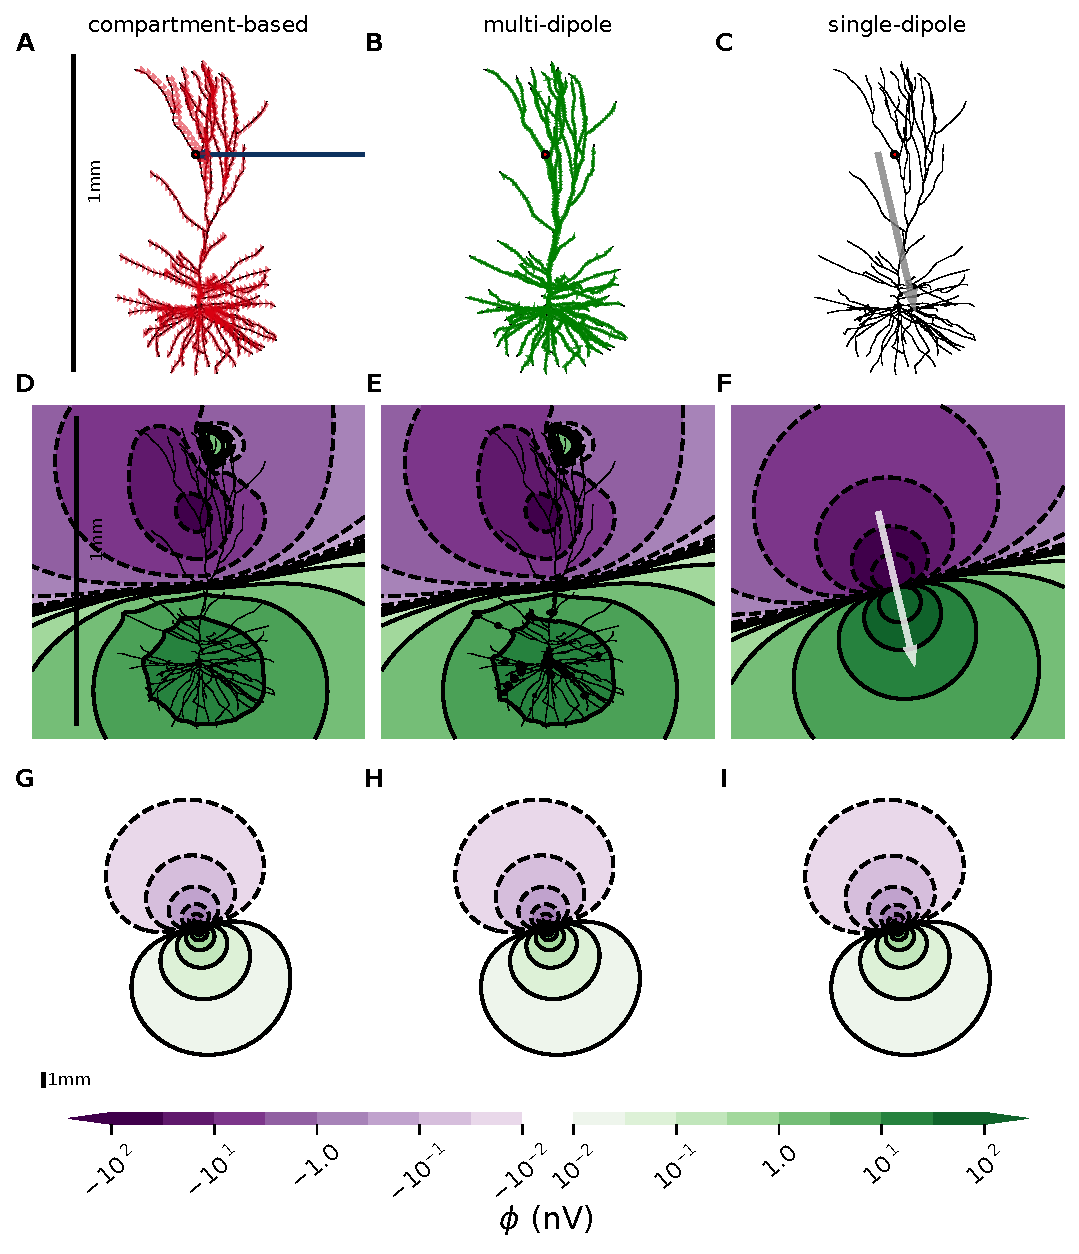
\includegraphics[width=1.0\textwidth]{fig_dipole_field_passiveTrue_single_syn481}
		\caption{\textbf{Extracellular potentials become dipolar in the far field limit}. 
			\textbf{A}: Layer 2/3 pyramidal cell from human \citep{EYAL2016} with an excitatory synapse placed on apical dendrite (red dot), and the resulting transmembrane currents for each compartment (blue and red arrows for negative and positive currents respectively).
			\textbf{B}: Green arrows represent the multiple current dipole moments between neighboring neural compartments.
			\textbf{C}: Gray arrow illustrates the total current dipole moment, that is, the sum of the dipoles in B.
			\textbf{D-F}: Extracellular potential in immediate proximity of the neuron, computed with the compartment-based approach, multi-dipole approach and single-dipole approximation, respectively. Note that the multi-dipole results differ slightly from the compartment-based approach when the distance from the measurement point to the nearest current dipole moment is short compared to the dipole length.
			\textbf{G-I}: Same as D-F, but at a larger spatial scale (zoomed out). See $1$~mm scalebar in panel A, D and G.
			\snnote{New synapse location with less dipol-shaped potential. Here, xlim and ylim are equal for first and second row, i.e. second row is more zoomed in than before. Don't know why the scalebars in A and D don't align. Will look into it. }
		}
		\label{fig:dipole_field}
	\end{figure}
	
	
	\subsection{Single-dipole approximation is justified for EEG, but not ECoG signals}\label{subsec:cb_db_comp_4s}
	
	%The ECoG and EEG signals are strongly affected by the very different conductivities of the CSF, skull and scalp \citep{NUNEZ2006}, and therefore, to test the applicability of the single-dipole approximation for computing ECoG and EEG signals, we used the four-sphere head-model \citep{NAESS2017, HAGEN2018, HAGEN2019}.
	%
	%For different positions of a single conductance-based excitatory synaptic input to the human cortical layer-2/3 pyramidal cell model \citep{EYAL2016}
	%(Fig.~\ref{fig:compare_multi_single_dipole}\textbf{A}), we calculated the electric potential from the top of the cell to the top of the head, using both the multi-dipole approach and the single-dipole approximation (Fig.~\ref{fig:compare_multi_single_dipole}\textbf{B}). As expected we found that synaptic input to the distal apical dendrite gave larger potentials than synaptic input to the proximal apical dendrite due to the larger current dipole moment \citep{LINDEN2010, AHLFORS2015}, and that in both cases the potential was strongly attenuated by crossing the different layers of the head model, most strongly across the low-conducting skull (Fig.~\ref{fig:compare_multi_single_dipole}\textbf{B}). 
	%
	%We observed only small differences between the multi-dipole approach and the single-dipole approximation for the distal synaptic input, while for the proximal synaptic input we observed a substantial difference directly above the cell model, that was decreased along the path towards the top of the head (Fig.~\ref{fig:compare_multi_single_dipole}\textbf{B}). We quantified these differences by looking at the relative error, and found that for the distal synaptic input the relative error was 1.23\% and 0.12\% at the position of the ECoG and EEG electrodes respectively, while for the proximal synaptic input the relative error was 39.4\% and 3.36\% at the position of the ECoG and EEG electrodes respectively (Fig.~\ref{fig:compare_multi_single_dipole}\textbf{C})
	%%\tvnnote{Solveig: Can you find exact numbers here?}. 
	%
	%In other words, the single-dipole approximation results in substantial errors at the position of the ECoG electrodes in both cases, but appears well-justified at the position of the EEG electrodes for some synaptic locations. In fact, we found that the relative error of the single-dipole approximation was strongly increased for synaptic locations $\sim$ 300~$\si{\um}$ above the soma (Fig.~\ref{fig:compare_multi_single_dipole}\textbf{D}). 
	%This point can be considered a 'center-of-gravity' for the cells transmembrane currents  \citep{LINDEN2010, AHLFORS2015}, meaning that for a synaptic input at this location, equally much of the return current will be above and below the synaptic input, resulting in a very weak current dipole moments (Fig.~\ref{fig:compare_multi_single_dipole}\textbf{E}).
	%This demonstrates that the relative error of the single-dipole approximation is negatively correlated with the amplitude of the current dipole moment (Fig.~\ref{fig:compare_multi_single_dipole}\textbf{F}), indicating that for large numbers of synaptic input, the total error of the single-dipole approximation can be expected to be small.
	
	
	The ECoG and EEG signals are strongly affected by the very different conductivities of the CSF, skull and scalp \citep{NUNEZ2006}. To implement the different conductivities into our calculations, we applied the four-sphere head model when testing the applicability of the single-dipole approximation for computing ECoG and EEG signals \citep{NAESS2017, HAGEN2018, HAGEN2019}.
	
	Our virtual experimental set-up consisted of a vertical electrode array placed directly above a single neuron. The electrode extended from 100 $\mu$m above the top of the neuron and all the way to the scalp surface.
	For different positions of a single conductance-based excitatory synaptic input to the human cortical layer-2/3 pyramidal cell model \citep{EYAL2016} \sntxt{with passive ion channels only}
	(Fig.~\ref{fig:compare_multi_single_dipole}\textbf{A}), we calculated the electric potential at the electrode measurement locations, using both the multi-dipole approach and the single-dipole approximation (Fig.~\ref{fig:compare_multi_single_dipole}\textbf{B}).
	
	
	As expected, we found that synaptic input to the distal apical dendrite gave larger potentials than synaptic input to the proximal dendrite, since the former leads to stronger current dipole moments \citep{LINDEN2010, AHLFORS2015}. For both synaptic input areas, the potential attenuated steeply with distance
	%\tvnnote{maybe 'steeply with distance' so it does not sound like we are talking about time?}
	when crossing the different layers of the head model, most strongly across the low-conducting skull (Fig.~\ref{fig:compare_multi_single_dipole}\textbf{B}). 
	
	\sntxt{We observed differences between the multi-dipole approach and the single-dipole approximation for distal  and proximal synaptic input, see green and purple lines in Fig.~\ref{fig:compare_multi_single_dipole}\textbf{B}, respectively.} %For the proximal synapses, on the other hand, we found a substantial difference directly above the cell model.
	These difference did, however, decrease along the path towards the top of the head. %(Fig.~\ref{fig:compare_multi_single_dipole}\textbf{B}, purple lines).
	We quantified the model dissimilarities by looking at the relative error, and found that for the distal synaptic input the relative error was 40.0\% and 1.06\% at the position of the ECoG and EEG electrodes respectively. Proximal synaptic input gave a relative error of 75.3$\%$ at the ECoG position, and 7.32$\%$ at the EEG position, (Fig.~\ref{fig:compare_multi_single_dipole}\textbf{C}).
	%\tvnnote{Solveig: Can you find exact numbers here?}. 
	In other words, the single-dipole approximation can result in substantial errors at the position of the ECoG electrodes, but appears well-justified at the position of the EEG electrodes for some synaptic locations. In fact, we found that the relative error of the single-dipole approximation \sntxt{peaked at synaptic locations $\sim$ 60 and 400~$\si{\um}$}
	%\tvnnote{from the figure, it looks more like 100 um up to 300 um?}
	above the soma (Fig.~\ref{fig:compare_multi_single_dipole}\textbf{D}). 
	\sntxt{\sout{This point} These points} can be considered \sntxt{\sout{s}} 'center\sntxt{s}-of-gravity' for the cell's transmembrane currents \citep{LINDEN2010, AHLFORS2015}, meaning that a synaptic input at \sntxt{\sout{this location}these locations} will lead to equal amounts of current returning above and below the synapse, resulting in very weak current dipole moment\sntxt{s} (Fig.~\ref{fig:compare_multi_single_dipole}\textbf{E}).
	This demonstrates that the relative error of the single-dipole approximation is negatively correlated with the amplitude of the current dipole moment (Fig.~\ref{fig:compare_multi_single_dipole}\textbf{F}), indicating that for large numbers of synaptic input, the total error of the single-dipole approximation can be expected to be small.
	\snnote{Do you think the above sentences still are ok, even though the trend is not as clear anymore?}
	Similar results were found for simulations with current-based synapses, and when including active ion channels.
	
	
	%We tested the applicability of the single-dipole model for computing ECoG and EEG signals, using the inhomogeneous four-sphere head-model. Since the four-sphere model takes current dipole moments as input, the multi-dipole model was used as ground truth. The Hay cell with conductance-based  exponential synaptic input was modeled with $30$ different input locations. Panel \textbf{D} of Figure~\ref{fig:compare_multi_single_dipole} show that apical synaptic input gives the largest current dipole moments. Moreover, panel \textbf{E} and \textbf{F} illustrate how relative errors for single-dipole model decay as function of dipole strength for ECoG and EEG signals. From panel \textbf{B} and \textbf{C} we can see how electric potential and relative error of single-dipole model fall as a function of distance from top of neuron to measurement electrode. The relative errors of the single-dipole model are higher for ECoG than for EEG signals. \snnote{give some example here!}
	%\tvnnote{Did we also try current-based synapse? I think we should, so we can say it didn't matter.}
	%\snnote{Did run. Didn't matter. Think we concluded that we don't need to mention this.}
	%\snnote{Mention in methods.}
	\begin{figure}[H]
		\centering
		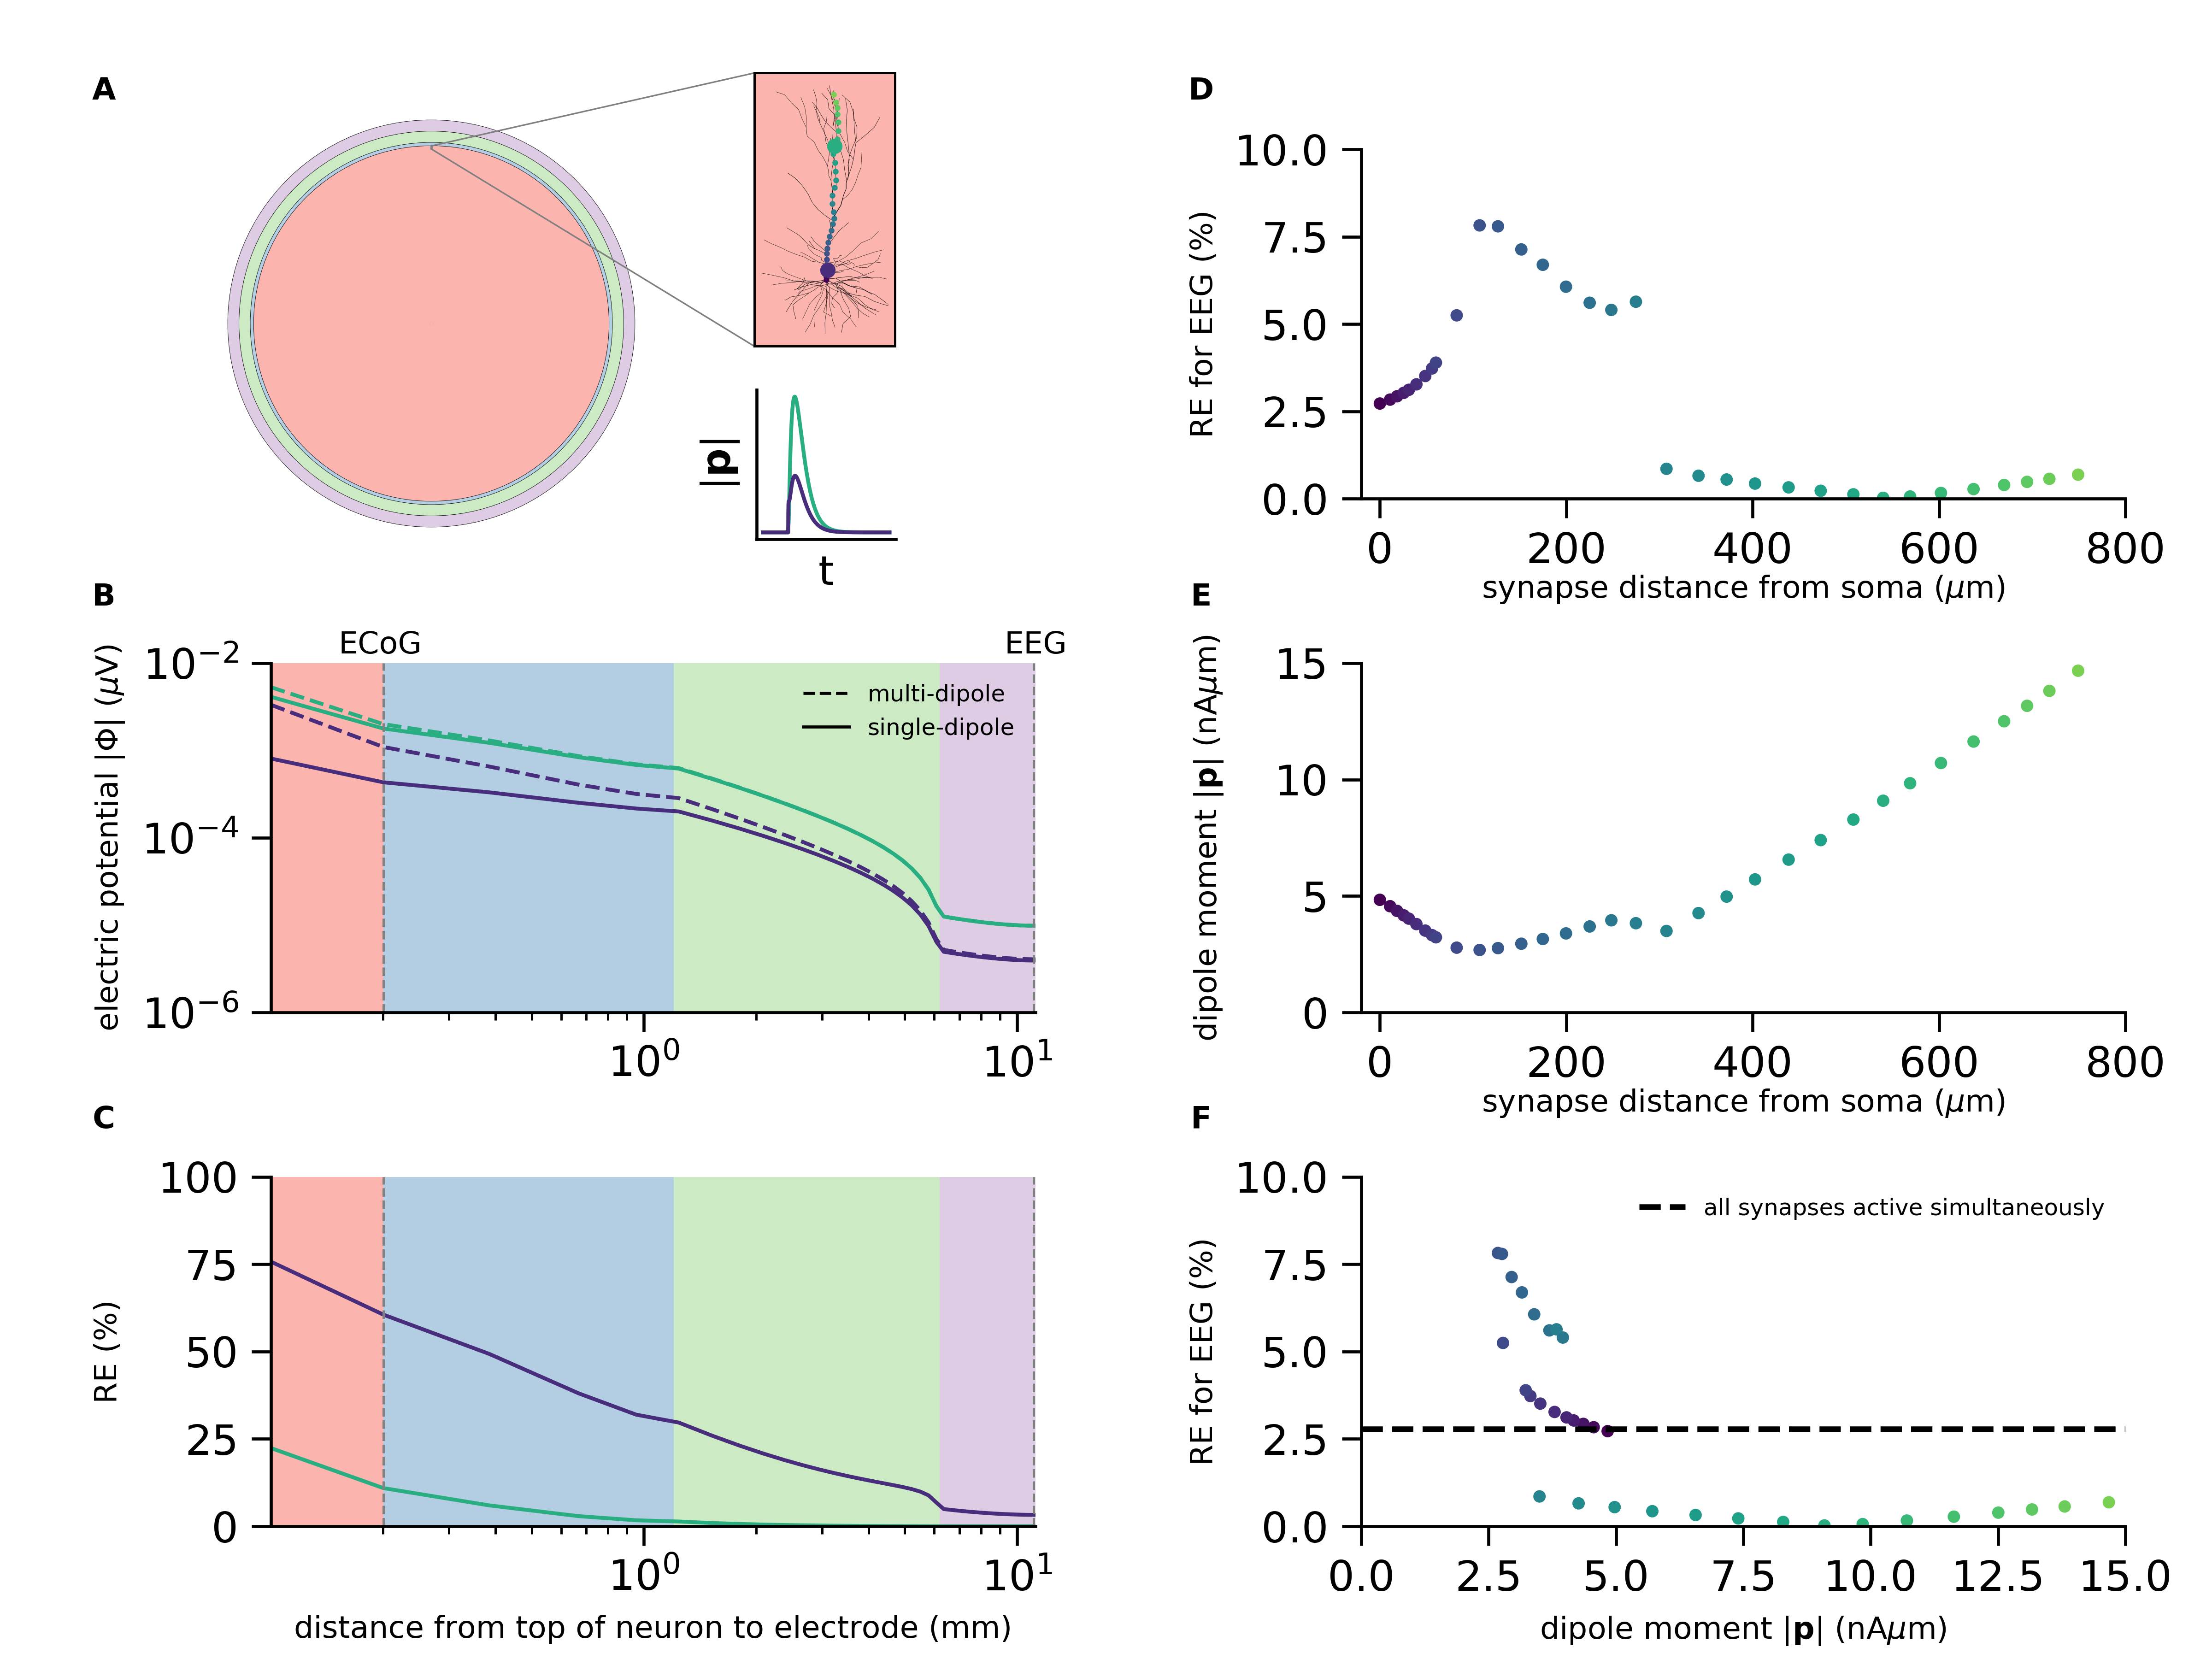
\includegraphics[width=1.0\textwidth]{figure2.png}
		\caption{\textbf{Single-dipole approximation is justified for EEG but not ECoG signals}. 
			\textbf{A}: Illustration of four-sphere head model, where the pink, blue, green and purple spherical shells represent the brain, CSF, skull and scalp respectively. The pink inset shows the human layer-2/3 neuron \citep{EYAL2016}. $41$ simulations lasting 100 ms with a single synaptic input after 20 ms to cell with passive ion channels only, were performed for varying input locations, see colored dots. \sntxt{The z-component of the resulting current dipole moments for two synaptic input locations (large colored dots) are shown in inset below as functions of time. The data presented in this figure are computed at the simulation time points producing the largest current dipole moment for each synaptic input location.}
			\textbf{B}: Magnitude of extracellular potential $|\phi|$ as function of distance from the top of the neuron, shown for two simulations with synaptic input locations marked by large colored dots in upper inset of A. In each simulation, we consider the timepoint with the largest current dipole moment. Dashed lines show extracellular potentials computed with multi-dipole, and full lines show single-dipole calculations.
			%\tvnnote{Is the potential at a given timestep, or is it max? Should be mentioned here I think.}
			\textbf{C}: Relative error RE at EEG location comparing the single-dipole model to the multi-dipole model, as function of distance from top of neuron to measurement point.
			\textbf{D}: Relative error RE showing how single-dipole model deviates from multi-dipole model EEG calculations, as function of distance from soma to synapse location.
			\textbf{E}: Magnitude of current dipole moment $|\mathbf{p}|$ as function of distance from soma to synaptic input location.
			\textbf{F}: Relative error RE showing how EEG calculations performed with the single-dipole approximation deviates from multi-dipole modeling results as function of magnitude of current dipole moment $|\mathbf{p}|$.
			%	\tvnnote{Suggestion: How about running another simulation with all synapses active simulataneously, calculate the relative error, and add it to this panel (F) as a horizontal line? We would expect this to give a small error, helping to illustrate our point of the EEG being dominated by low-error dipoles.}
			\gtenote{I wonder if it could be an idea to have a panel illustrating the timecourse of the signal underlying these results?}
			\snnote{inset in A ok?}
		}
		%	\tvnnote{Suggestion: How about running another simulation with all synapses active simulataneously, calculate the relative error, and add it to this panel (F) as a horizontal line? We would expect this to give a small error, helping to illustrate our point of the EEG being dominated by low-error dipoles.}
		\label{fig:compare_multi_single_dipole}
	\end{figure}
	
	\subsection{Compact description of EEG contribution simplifies analysis}\label{subsec:compact}
	%In the previous section we showed that the single-dipole approximation was applicable for calculation of EEG signals from a single synaptic input to a human cortical Layer 2/3 cell model, and we now expand this to three different cell types (Fig.~\ref{fig:eeg_compare_cell_types}\textbf{A}), each receiving a large number of synaptic inputs arriving in waves with specific target regions on the cells (Fig.~\ref{fig:eeg_compare_cell_types}\textbf{B}).
	In the previous section we showed that the single-dipole approximation was applicable for calculation of EEG signals, and in this section we demonstrate that the single-dipole approximation can substantially simplify the analysis of the biophysical origin of EEG signals.
	
	\subsubsection{Single-dipole approximation simplifies estimate of EEG contribution}
	
	Pyramidal cells have a preferred orientation along the depth axis of cortex (here the $z$-axis), and the direction of the current dipole moment $\mathbf{p}$ can be expected to align with this axis since
	radial symmetry will tend to make the orthogonal components ($p_x$, $p_y$) cancel \citep{HAGEN2018}. 
	In contrast, interneurons show much less of a preferred orientation, and are therefore not expected to give any meaningful contribution to the EEG signal, except indirectly through input to pyramidal cells \citep{HAGEN2016}.
	We illustrated this by applying the single-dipole approximation to three different cell types (Fig.~\ref{fig:eeg_compare_cell_types}\textbf{A}), each receiving a large number of synaptic inputs arriving in waves with specific target regions on the cells (Fig.~\ref{fig:eeg_compare_cell_types}\textbf{B}). The synaptic input weights for all synapses of the same type (excitatory/ inhibitory) in a single wave, summed to 0.01.
	
	For the previously used human layer-2/3 cell (Fig.~\ref{fig:eeg_compare_cell_types}\textbf{A}, purple; \cite{EYAL2016}),
	receiving a wave of 100 excitatory synaptic inputs that were restricted to the uppermost 200~$\si{\um}$ of the cell (time=50~ms; Fig.~\ref{fig:eeg_compare_cell_types}\textbf{B}, purple dots), we observed a negative deviation of $p_z$ (Fig.~\ref{fig:eeg_compare_cell_types}\textbf{C}, purple line). For basal synaptic input (time=100~ms; Fig.~\ref{fig:eeg_compare_cell_types}\textbf{B}, purple line), the polarity of $p_z$ was instead positive, but of slightly lower amplitude than for apical input, as can be expected because the large area of the somatic region will cause strong return currents in the immediate vicinity of the synaptic inputs, and therefore an overall weaker current-dipole moment.
	
	
	A uniform distribution of 400 synaptic inputs across the cell membrane with area-weighted probability (time=150~ms; Fig.~\ref{fig:eeg_compare_cell_types}\textbf{B}, purple line), only gave rise to small ripples in $p_z$, due to the substantial cancellation of current dipoles of opposite polarity. It is sometimes assumed that excitatory input is relatively uniformly distributed onto pyramidal cells, while inhibitory input is more directed to the perisomatic region (cite Pablo when published \citep{Mazzoni2015, Skaar2020}). As expected, we found that the combination of the previously described wave of uniformly distributed excitatory synaptic input, combined with perisomatic inhibitory inputs gave rise to a clear negative response in $p_z$ (time=200~ms; Fig.~\ref{fig:eeg_compare_cell_types}\textbf{B}, purple line), which could be part of the explanation why inhibitory synaptic input in some cases have been found to dominate the LFP \citep{HAGEN2016, TELENCZUK2016}.
	
	For a rat cortical layer-5 pyramidal cell model (Fig.~\ref{fig:eeg_compare_cell_types}\textbf{A}, blue; \cite{HAY2011}) \sntxt{\sout{with 10 active conductances and capability for both somatic and dendritic spikes (note that for now the synaptic input was subthreshold)}}, the resulting current dipole moment was very similar in shape, but larger in amplitude, which was expected because the longer apical dendrite will tend to give larger current dipole moments (Fig.~\ref{fig:eeg_compare_cell_types}\textbf{C}, blue line).
	
	Lastly, we used a rat cortical layer-5 interneuron model (Fig.~\ref{fig:eeg_compare_cell_types}\textbf{A}, green; \cite{MARKRAM2015}), but since the dendrites of interneurons are not structured into the same distinctive zones as pyramidal cells, \sntxt{\sout{ all synaptic input was uniformly distributed, and therefore} the synaptic input} caused very small net current dipole moments.
	%\snnote{For the interneuron, the input is actually distributed such that apical means above z = 0, and basal means below z = 0. This does perhaps not make sense biologically.. Would it be better to have uniform distribution for both "apical", "basal" and "uniform"?}
	\sntxt{\sout{From all three cell models w} W}e calculated the EEG signal\sntxt{s} with the four-sphere head model, using both the multi-dipole (Fig.~\ref{fig:eeg_compare_cell_types}\textbf{D}, dotted lines) and the single-dipole (Fig.~\ref{fig:eeg_compare_cell_types}\textbf{D}, solid lines) approach. \sntxt{The maximum global error was below 3.5$\%$ for all cells.
		%\sout{In all three cases, we found the single-dipole approximation to be in excellently agreement with the multi-dipole approach, demonstrating that}  
		Importantly, }
	%\sntxt{The resulting EEG signals modeled with the four-sphere head model is shown in Fig.~\ref{fig:eeg_compare_cell_types}. We applied both the multi-dipole (dotted line) and the single dipole model (solid line).} \snnote{maximum global error is 1.5$\%$ for Segev, 2.7$\%$ for Hay and 49$\%$ for interneuron. Don't know if we should include these numbers. It seems like these maximum errors occur for apical input, while in fig. 2 the largest errors followed basal input..}
	%Note that in all cases, 
	the EEG signal is nearly fully described by the single-dipole $p_z$, that is, a single time-dependent array, which corresponds to a massive simplification in understanding the biophysical origin of the EEG signal, compared to considering the transmembrane currents and position of each cellular compartment. 
	
	%We found in the previous section that the single-dipole approximation was applicable for calculation of EEG signals, but we have not yet demonstrated its usefulness for modeling and understanding the EEG.
	
	%\tvnnote{Solveig: Could you perhaps run the simulations in Figure 3 with the multi-dipole approach as well, so we can look at the error for the different waves and cells? I'm not sure it needs to be in the figure, but it would be good to give a maximum relative error I think ('relative' with respect to the maximum signal: error / max(abs(sig))). When writing this, it feels like our verification is a bit weak still.
	%Maybe it would make sense to add the multi-dipole EEG as dashed lines in panel D as well?
	%}
	%\snnote{Jepp!}
	%\snnote{still not certain about the second-to-last sentence. How about just going for your striked-out alternative, but skip "excellently"? I think that would be less confusing. Then we could include all the errors in the caption instead?}
	
	\begin{figure}[H]
		\centering
		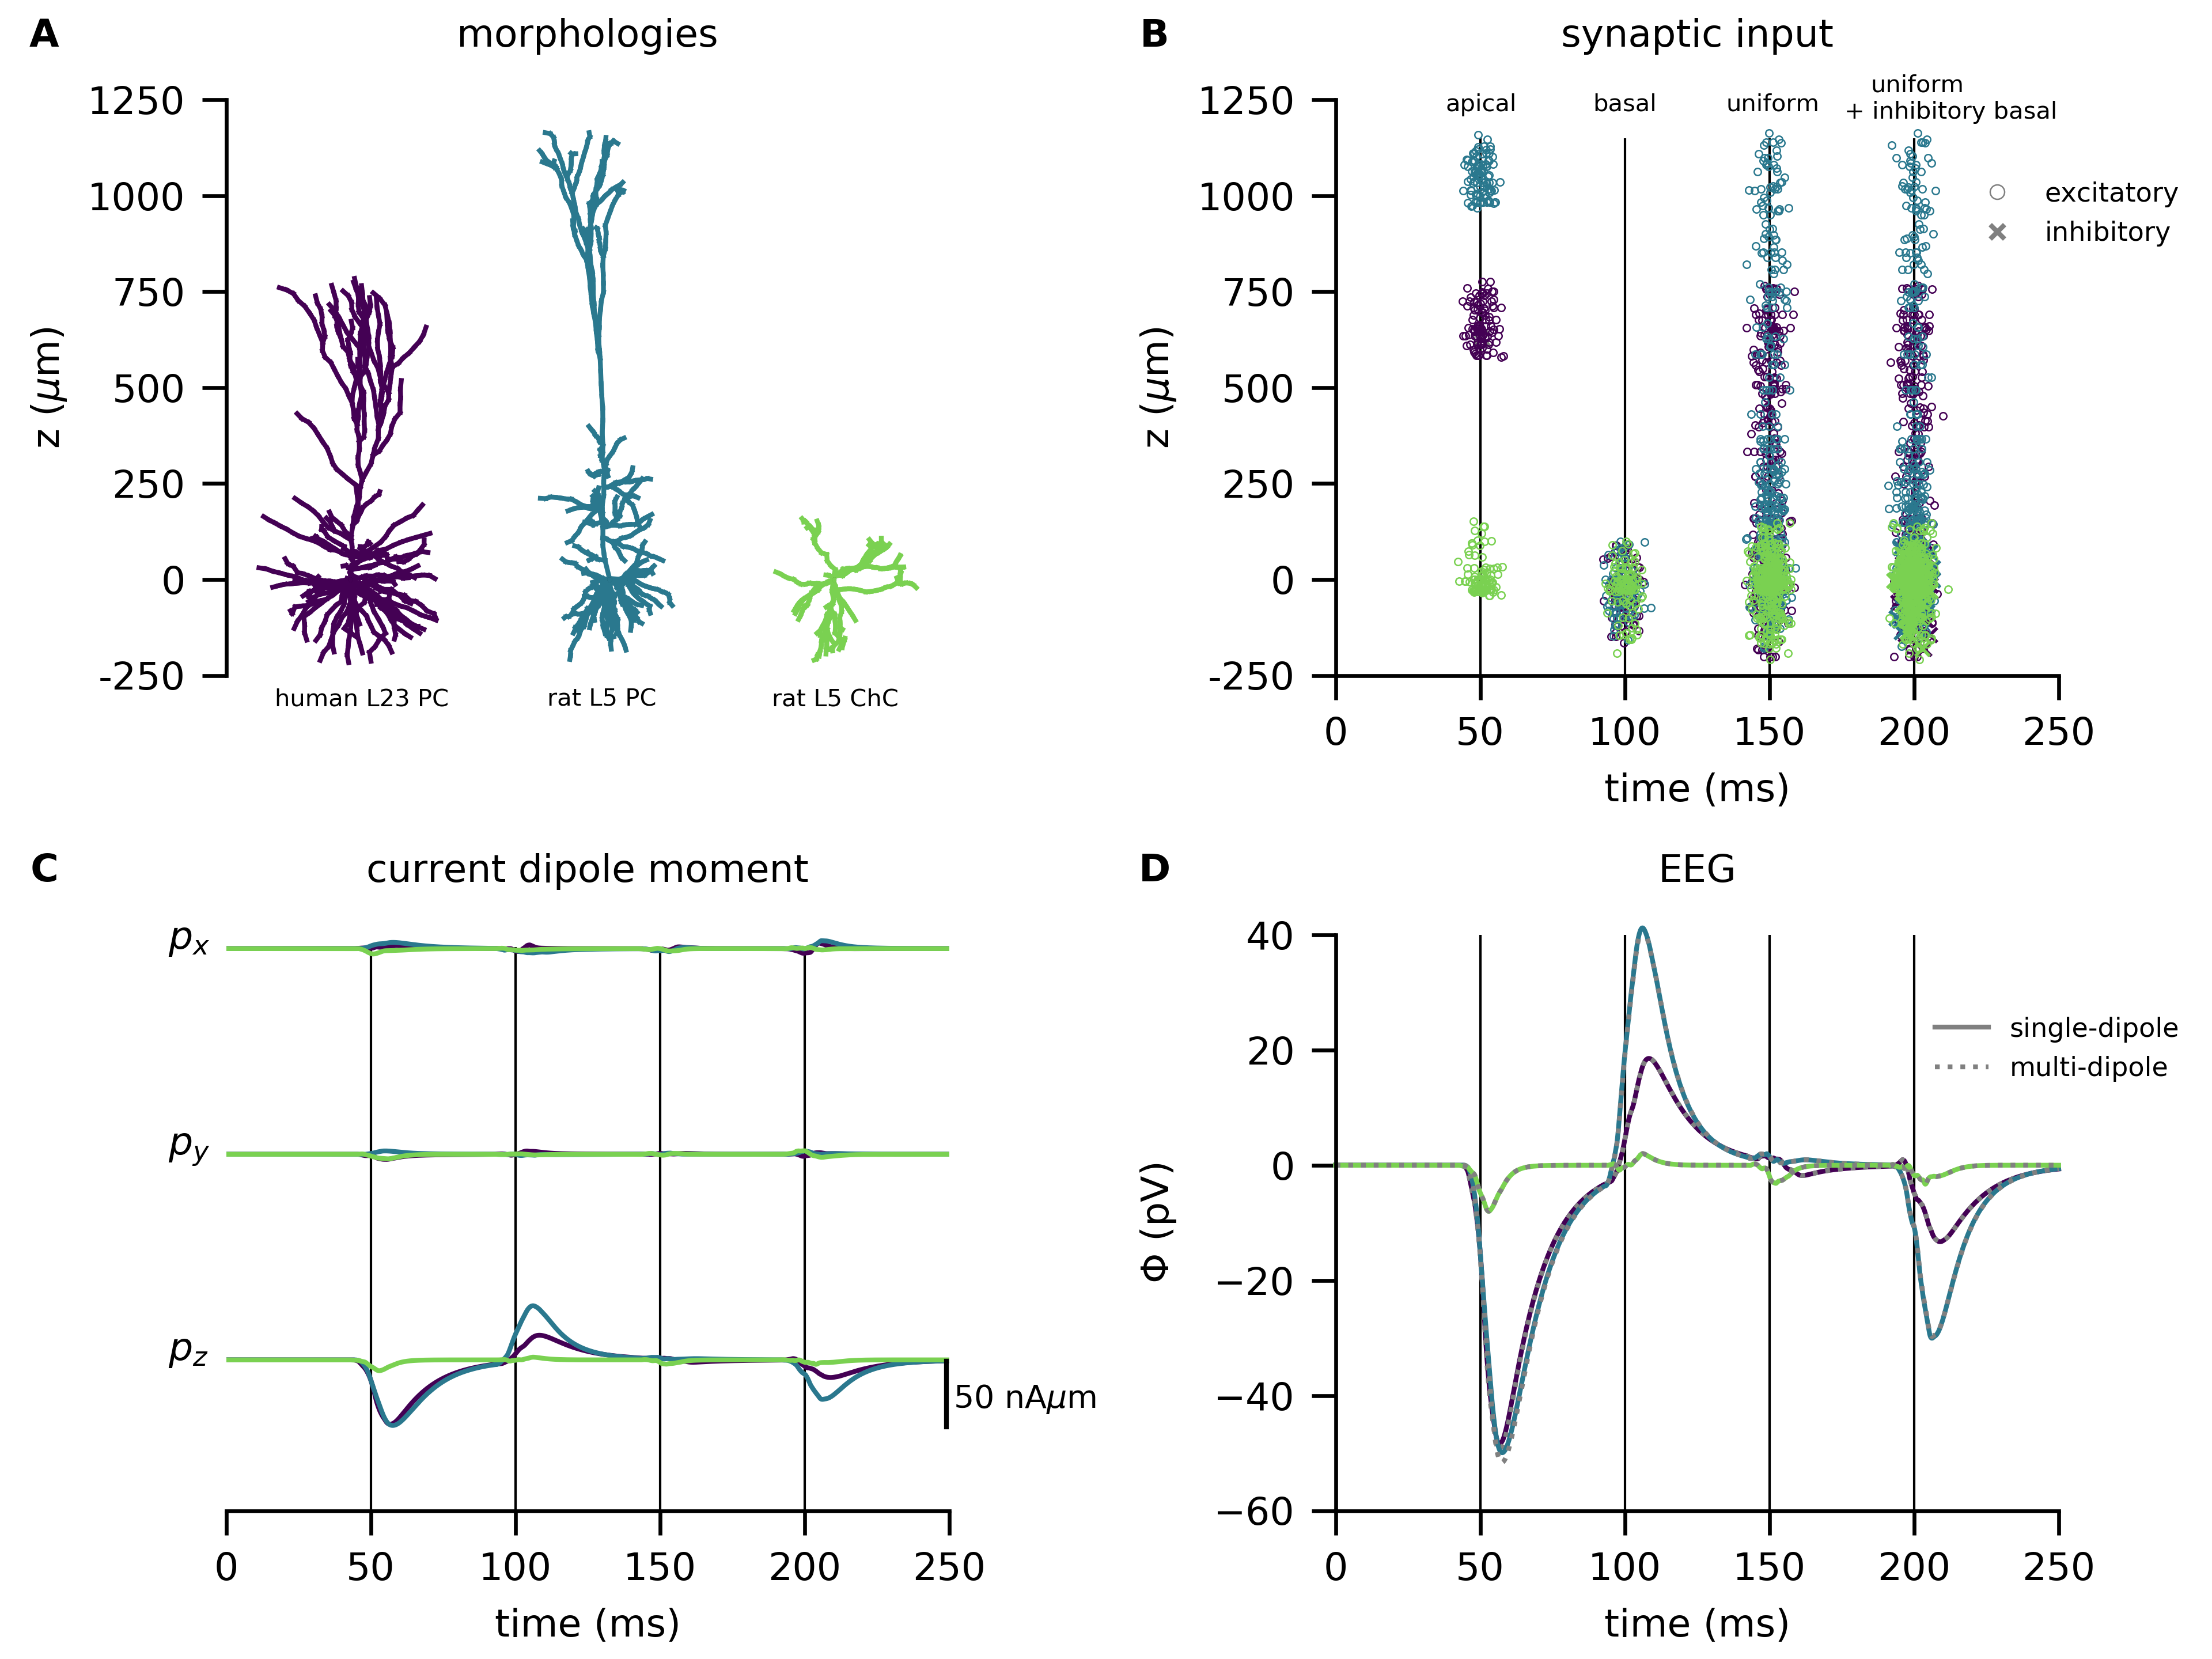
\includegraphics[width=0.8\textwidth]{figure3.png}
		\caption{\textbf{EEG signals and current dipole moment from three different cell types with various synaptic input}.
			\textbf{A}: The morphologies of a human L2/3 pyramidal cell (purple; \cite{EYAL2016}), a rat L5 pyramidal cell (blue; \cite{HAY2011}), and a rat L5 interneuron (green; \cite{MARKRAM2015}). All panels use the same colors for data from each cell type.
			\textbf{B}: Each dot represents an excitatory synaptic input at a specific time (x-axis) at a specific height of the neuron (z-axis, corresponding to panel A) for a specific cell type (color). The crosses mark inhibitory synaptic input. The four input bulks represent 1) 100 apical excitatory synapses, 2) 100 basal excitatory input, 3) 400 homogeneously spread-out excitatory synapses and 4) 400 homogeneously spread-out excitatory synapse and inhibitory basal synapses. The synaptic weights summ to 0.01 for all sets of excitatory/ inhibitory synapses in each wave.
			\textbf{C}: The x-, y- and z-components of the current dipole moment $\mathbf{p}$ for the three different cell types.
			\textbf{D}: EEG signals, $\phi$ from the three cell types computed with the four-sphere model.
		}
		\label{fig:eeg_compare_cell_types}
	\end{figure}
	
	
	\subsubsection{Current dipole moment expose dendritic calcium spikes}
	
	%\cite{SUZUKI2017} recently demonstrated that dendritic calcium spikes could be recorded at the cortical surface with amplitudes of similar magnitude as the contribution from synaptic inputs. This demonstrates that active conductances may play an important role in shaping ECoG and EEG signals, and also suggests that information might be present in such signals which can be used in new ways to study the learning mechanisms associated with dendritic calcium spikes (cite). We found that the single-dipole approximation provides a convenient way of investigating the EEG-contribution of such dendritic calcium spikes.
	%
	%The previously introduced rat layer 5 cortical pyramidal cell model from \cite{HAY2011} can exhibit dendritic calcium spikes.
	%When this cell model received a single excitatory synaptic input to the soma (Fig.~\ref{fig:ca_spike}\textbf{A}, blue dot) strong enough to elicit a somatic action potential (Fig.~\ref{fig:ca_spike}\textbf{B1}, blue), a small depolarization was also visible in the apical dendrite but no dendritic calcium spike was initiated (Fig.~\ref{fig:ca_spike}\textbf{B1}, orange). If instead the same somatic synaptic input was combined with an additional excitatory synaptic input to the apical dendrite 400~$\si{\um}$ away from the soma (Fig.~\ref{fig:ca_spike}\textbf{A}, orange dot), a dendritic calcium spike was initiated, which also induced two additional somatic spikes (Fig.~\ref{fig:ca_spike}\textbf{C1}).
	%
	%The simulated extracellular potential 30~$\si{\um}$ away from the soma had the shape of stereotypical extracellular action potentials in both cases, that is, a sharp negative peak followed by a broader and weaker positive peak (Fig.~\ref{fig:ca_spike}\textbf{B2, C2}), and the slow dendritic calcium spike was not reflected in the extracellular potential close to the soma (Fig.~\ref{fig:ca_spike}\textbf{C2}).
	%We found that for the case with only a somatic spike and no calcium spike, the single-cell current dipole moment resembled the inverse of the extracellular potential (Fig.~\ref{fig:ca_spike}\textbf{B3}), while for the case with both somatic and dendritic spiking, a pronounced slow component was also present in the single-cell current dipole moment (Fig.~\ref{fig:ca_spike}\textbf{C3}).
	%Note that somatic action potentials are typically not expected to contribute significantly to EEG signals (cite, but see \cite{TELENCZUK2015}), because the very short duration of spikes with both a positive and a negative phase implies that extreme synchrony is needed for spikes to sum constructively. Indeed, we found that when we calculated the sum of 1'000 instanced of the single-cell current dipole moment that was jittered (shifted) in time (normally distributed, standard deviation=10~ms), the case with the dendritic calcium spike has a $6.6$-fold larger maximum amplitude than the case with
	%only the somatic spike (Fig.~\ref{fig:ca_spike} \textbf{B4} versus \textbf{C4}, 
	%$\mathrm{max}|\mathbf{p}$| = 30.8~$\si{\uA}\cdot\si{\um}$ and 204.2~$\si{\uA}\cdot\si{\um}$ respectively). This demonstrates that dendritic calcium spikes are much more capable of summing constructively for a population of cells, and substantiates the role of dendritic calcium spikes in affecting ECoG/EEG/MEG recordings. 
	%\tvnnote{Although our Ca-spikes appear quite different in shape to the ones demonstrated by Suzuki and Larkum (2017), who (in defence of our results) reported an 'unexpected shape'}
	%
	%It might initially seem surprising that the dendritic calcium spike is so strongly reflected in the single-cell current dipole moment, given that the transmembrane currents associated with the somatic action potential are much larger than those associated with the dendritic calcium spike: the maximum amplitude of the transmembrane currents of the somatic compartment was 45.1~$\si{\nA}$, compared to just 0.30~$\si{\nA}$ for the compartment with the apical synaptic input (Fig.~\ref{fig:ca_spike}A, blue and orange dots). However, the current dipole moment is given as the product between the amplitude of the current and the separation between the source and sink ($\mathbf{p}=I\mathbf{d}$; eq. \ref{eq:dip_trans_to_axial}), and while the currents associated with the somatic action potential will for the most part be contained within the somatic region, giving very small sink/source separations, the currents associated with the dendritic calcium spike will be distributed over a much larger part of the cell membrane (cite?).
	
	\cite{SUZUKI2017} recently demonstrated that dendritic calcium spikes can be recorded at the cortical surface, and that the signal amplitudes can be similar to contributions from synaptic inputs.
	%\snnote{I neste setning skjonner jeg ikke helt hva "which" refererer til: signals eller information? } \tvnnote{better now?}
	%This demonstrates that active conductances may play an important role in shaping ECoG and EEG signals, and also suggests that information might be present in such signals which can be used in new ways to study the learning mechanisms associated with dendritic calcium spikes (cite). 
	This demonstrates that active conductances may play an important role in shaping ECoG and EEG signals. Furthermore, it suggests that information about calcium dynamics might be present in such signals, and \sntxt{\sout{such} that this} information could potentially be taken advantage of \sntxt{\sout{for} when} studying learning mechanisms associated with dendritic calcium spikes (cite).
	%\tvntxt{\sout{We found that the single-dipole approximation provides a convenient way of investigating the EEG-contribution \sntxt{\sout{of} from} such dendritic calcium spikes.}}
	
	The previously introduced rat layer-5 cortical pyramidal cell model from \cite{HAY2011} can exhibit dendritic calcium spikes.
	When this cell model received a single excitatory synaptic input to the soma (Fig.~\ref{fig:ca_spike}\textbf{A}, blue dot), strong enough to elicit a somatic action potential (Fig.~\ref{fig:ca_spike}\textbf{B1}, blue), a small depolarization was also visible in the apical dendrite (Fig.~\ref{fig:ca_spike}\textbf{B1}, orange. Even so, this did not iniate any dendritic calcium spike. However, when combining the same somatic synaptic input with an additional excitatory synaptic input to the apical dendrite, 400~$\si{\um}$ away from the soma (Fig.~\ref{fig:ca_spike}\textbf{A}, orange dot),we observed a dendritic calcium spike. The calcium spike did, in turn, induce two additional somatic spikes (Fig.~\ref{fig:ca_spike}\textbf{C1}).
	
	For both synaptic input strategies described above, the extracellular potential simulated 30~$\si{\um}$ away from the soma took the shape of stereotypical extracellular action potentials: that is, a sharp negative peak followed by a broader and weaker positive peak (Fig.~\ref{fig:ca_spike}\textbf{B2, C2}). Further, we observed that the slow dendritic calcium spike was not reflected in the extracellular potential close to the soma (Fig.~\ref{fig:ca_spike}\textbf{C2}).
	We found that for the case with only a somatic spike and no calcium spike, the single-cell current dipole moment resembled the inverse of the extracellular potential (Fig.~\ref{fig:ca_spike}\textbf{B3}), while for the case with both somatic and dendritic spiking, a pronounced slow component was also present in the single-cell current dipole moment (Fig.~\ref{fig:ca_spike}\textbf{C3}).
	Note that somatic action potentials are typically not expected to contribute significantly to EEG signals (cite, but see \cite{TELENCZUK2015}), because the very short duration of spikes with both a positive and a negative phase implies that extreme synchrony is needed for spikes to sum constructively. Indeed, we found that when we calculated the sum of 1'000 instances of the single-cell current dipole moment that was jittered (shifted) in time (normally distributed, standard deviation=10~ms), the case with the dendritic calcium spike had a $6.6$-fold larger maximum amplitude than the case with
	only the somatic spike (Fig.~\ref{fig:ca_spike} \textbf{B4} versus \textbf{C4}, 
	$\mathrm{max}|\mathbf{p}$| = 30.8~$\si{\uA}\cdot\si{\um}$ and 204.2~$\si{\uA}\cdot\si{\um}$ respectively).
	%\snnote{It is hard to read these numbers out from the plots.. Something odd with the axes here?}
	This demonstrates that dendritic calcium spikes are much more capable of summing constructively for a population of cells, and substantiates the role of dendritic calcium spikes in affecting ECoG/EEG/MEG recordings. 
	%\tvnnote{Although our Ca-spikes appear quite different in shape to the ones demonstrated by Suzuki and Larkum (2017), who (in defence of our results) reported an 'unexpected shape'}
	
	It might initially seem surprising that the dendritic calcium spike is so strongly reflected in the single-cell current dipole moment, given that the transmembrane currents associated with the somatic action potential are much larger than those associated with the dendritic calcium spike: the maximum amplitude of the transmembrane currents of the somatic compartment was 45.1~$\si{\nA}$, compared to just 0.30~$\si{\nA}$ for the compartment with the apical synaptic input (Fig.~\ref{fig:ca_spike}{\bf A}, blue and orange dots). However, the current dipole moment is given as the product between the amplitude of the current and the separation between the source and sink ($\mathbf{p}=I\mathbf{d}$; Equation \ref{eq:dip_trans_to_axial}), and while the currents associated with the somatic action potential will for the most part be contained within the somatic region, giving very small sink/source separations, the currents associated with the dendritic calcium spike will be distributed over a much larger part of the cell membrane (cite?).
	
	\begin{figure}[H]
		\centering
		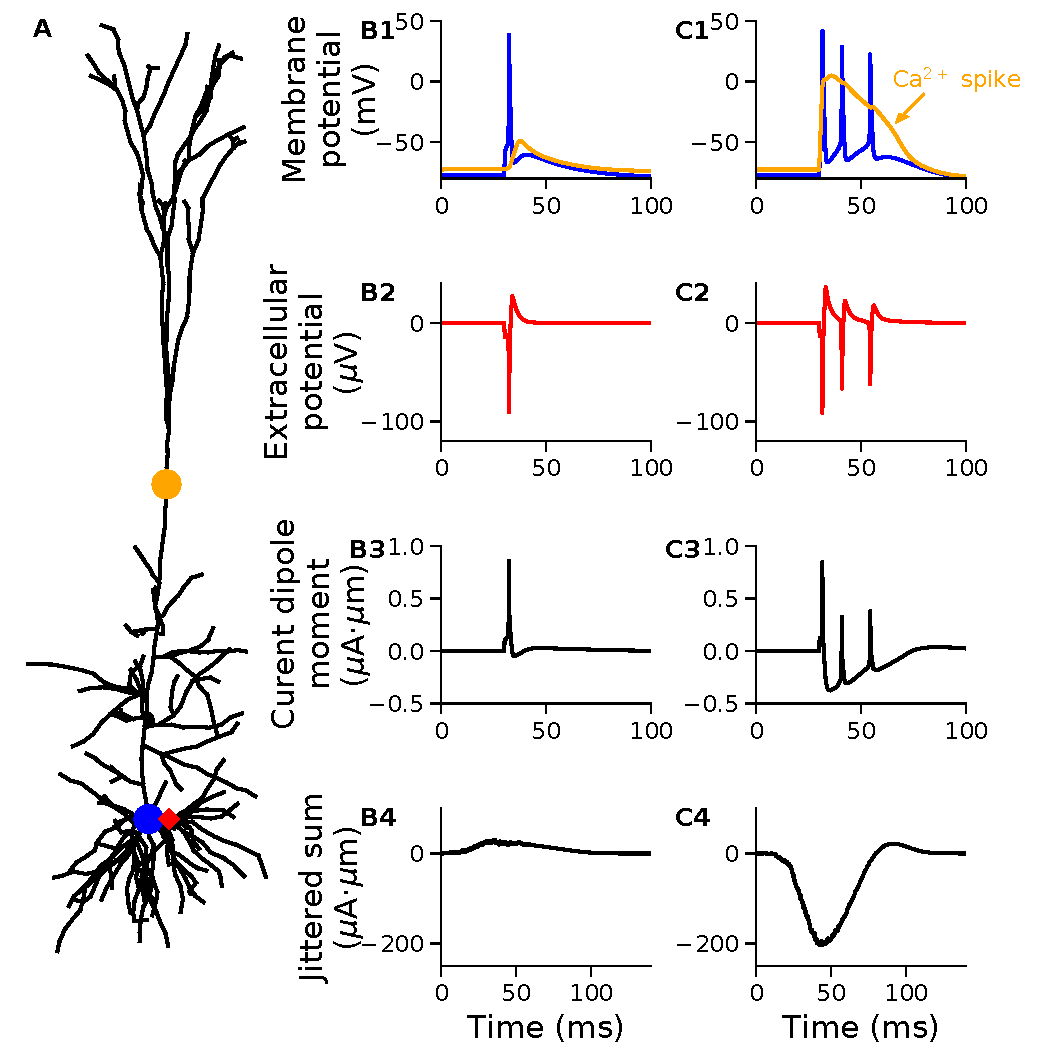
\includegraphics[width=0.6\textwidth]{ca_spike_hay}
		\caption{\textbf{Current dipole moment expose dendritic calcium spikes.}
			\textbf{A}: Layer 5 cortical pyramidal cell model from rat \citep{HAY2011}, receiving either a single excitatory synaptic input to the soma evoking a single somatic action potential (blue dot, results in \textbf{B1-4}), or in addition an excitatory synaptic input to the apical dendrite, evoking a dendritic calcium spike and two additional somatic spikes (orange dot, results in \textbf{C1-4}). 
			\textbf{B1, C1}: Membrane potential at the two positions indicated in \textbf{A}.
			\textbf{B2, C2}: Extracellular potential 30~$\si{\um}$ away from the soma (red diamond in \textbf{A}), assuming for illustration an infinite homogeneous extracellular medium. 
			\textbf{B3, C3}: Single-cell current dipole moment. 
			\textbf{B4, C4}: Sum of 1'000 instances of the single-cell current dipole moment (from \textbf{B3, C3}), that has been randomly shifted in time with a normally distributed shift with a standard deviation of 10~ms.
		}
		\label{fig:ca_spike}
	\end{figure}
	
	\subsection{Dipole approximation for populations of cells}\label{subsec:populations}
	So far, we have only considered the EEG contributions from single cells, but real EEG signals are expected to reflect the activity of hundreds of thousands to millions of cells \citep{NUNEZ2006, COHEN2017}. 
	%There are several ongoing large-scale modeling efforts that seek to simulate neural activity at different levels of biological detail. 
	Biophysically detailed modeling of large populations is still in its infancy \citep{EINEVOLL2019} and at present typically include ``only'' a few tens of thousands of biophysically detailed cells \citep{MARKRAM2015, BILLEH2019}. Networks of point neurons on the other hand are regularly used to simulate hundreds of thousands \citep{BILLEH2019} or even millions of cells \citep{SENK2018, SCHMIDT2018}, however, point-neurons in their nature lack the ability to predict LFP, ECoG, EEG or MEG signals \citep{EINEVOLL2013REVIEW}.  
	
	We therefore used the hybrid scheme \citep{HAGEN2016, SENK2018, Skaar2020}, where the network activity is first simulated in a highly computationally efficient manner with point neurons in NEST \citep{NEST} and the spiking activity of each neuron saved to file. Afterwards, each cell is modeled with biophysically detailed multicompartment morphologies, capable of predicting extracellular potentials, and the spikes of all the presynaptic neurons are used as synaptic input \citep{HAGEN2016, SENK2018}.
	
	We used the large-scale point-neuron cortical microcircuit model from \cite{POTJANS2014, HAGEN2016}, which has $\sim$80'000 neurons divided into 8 different cortical populations, one excitatory and one inhibitory across four layers (L2/3 - L6), and can exhibit a diverse set of spiking dynamics including different oscillations and asynchroneous irregular network states \citep{HAGEN2016, BRUNEL2000}. 
	The only difference from the original simulations by \cite{HAGEN2016} was the added calculation of current dipole moments.
	We simulated transient thalamic synaptic input to layers 4 and 6 (Fig.~\ref{fig:population}\textbf{A}), and after the spikes had been mapped onto the multicompartment cell models (Fig.~\ref{fig:population}\textbf{B}), we calculated the LFP (Fig.~\ref{fig:population}\textbf{B}) similarly to \cite{HAGEN2016} (their Fig.~1), in addition to the current dipole moments of each cell.
	
	
	For all cell populations, we found that the current dipole moment from individual cells could show large transient responses to thalamic input (Fig.~\ref{fig:population}\textbf{D}; gray lines show current dipole moment from individual cells in two example populations: L5 inhibitory (L5I) and L5 exitatory (L5E)), however, for all inhibitory populations the thalamic response was not visible in the average current dipole moment (Fig.~\ref{fig:population}\textbf{D}; black lines, L5I). The same was true for the current dipole moment components perpendicular to the depth axis for excitatory populations (Fig.~\ref{fig:population}\textbf{D}; L5E, $p_x, p_y$, black lines), but not for the component along the depth axis which had a substantial average response to the thalamic input (Fig.~\ref{fig:population}\textbf{D}; L5E, $p_z$, black line). 
	These observations imply that, as previously mentioned, only the z-component of the current dipole moment from excitatory populations can be expected to contribute significantly to the EEG signal.
	
	Our findings invite a simplified approach to calculate the EEG signal: Instead of calculating all single-cell EEG contributions and summing them (taking into account the position of the individual cells, similarly to what is done for the LFP signal), we can compute one summed $p_z$-component from each pyramidal cell population, place it in the population center, and calculate the resulting simplified EEG signal. This approximation is reasonable when the population radius is small compared to the distance from the population center to the EEG electrode. Note that the distance from the top of cortex to the top of the head is typically $\sim$10~mm, while the radius of the simulated population is here only $\sim$0.5~mm (Fig.~\ref{fig:population}; population outline in \textbf{B} is drawn in red in \textbf{E}).
	
	Indeed, when we combined the current dipole moments with the four-sphere head model (Fig.~\ref{fig:population}\textbf{E}), we found that the full EEG signal that was calculated as the sum of the EEG contribution from each of the $\sim$80'000 cells at their respective positions, was in fact indistinguishable from the simplified EEG signal (Fig.~\ref{fig:population}\textbf{F}). This implies that a full understanding of the EEG signal from simulated cortical activity can be extracted from a single time-dependent array for each pyramidal cell population (see Discussion for limitations).
	
	We also compared the relative amplitude of the EEG signal from each population, and found that in this case, the excitatory population of L2/3 was the dominant source of the EEG signal (Fig.~\ref{fig:population}\textbf{F}), in line with (?)\tvnnote{(cite!)}. Note, however, that we expect this observation to be somewhat model-dependent, and \sntxt{that?} making strong claims about the contribution of different pyramidal cell populations would require a more thorough analysis than the scope of this study allows.
	
	\begin{figure}[H]
		\centering
		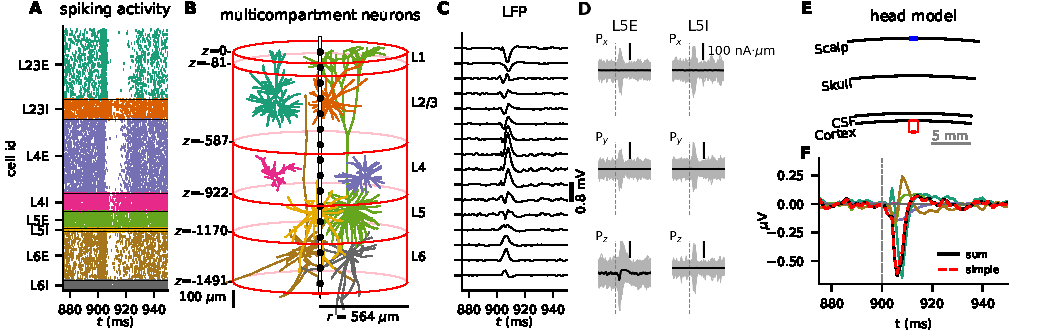
\includegraphics[width=1.0\textwidth]{hybrid_with_EEG}
		\caption{\textbf{Large-scale neural simulations can be used to probe biophysical origin of EEG signals}. 
			\textbf{A}: Stimulus-evoked spiking activity from thalamic input (time $t= $ 900~ms, denoted by thin vertical line) in the cortical microcircuit model from \cite{POTJANS2014}. Dots indicate spike times of individual neurons, and populations are represented in different colors (I=inhibitory, E=excitatory).
			\textbf{B}: Multicompartment model neurons used to produce the measurable signals, with colors corresponding to panel \textbf{A}, showing one example morphology per population. Layer boundaries are marked at depths relative to cortical surface, z = 0. A laminar recording electrode with 16 contacts separated by
			100 $\mu$m (black dots) is positioned in the center of the population.
			\textbf{C}: LFPs calculated at depths corresponding to black dots in \textbf{B}.
			\textbf{D}: For the two L5 populations (L5I and L5E), the three components of the current dipole moment is shown for all individual cells (gray), together with the population average (black).
			\textbf{E}: Illustration of the four-sphere head model, with the red column corresponding the the outline of the population in panel \textbf{B}.
			\textbf{F}: The EEG signal from each population found by summing the single-cell EEG contribution of all individual cells (different colors), together with the total summed EEG signal (black). The simplified EEG signal was found by first summing the z-component of the current dipole moments for all pyramidal cells, that is L2/3E, L5E and L6E, and calculating the EEG from this single current dipole (red dashed).
			\snnote{maybe we can align the panel lettering?}
		}
		\label{fig:population}
	\end{figure}
	
	
	\subsection{Dipole approximation in more complex head models}
	%The construction of such realistic head models are typically dependent on very expensive equipment, such as magnetic resonance imaging (MRI), to map the electrical conductivity of the entire head at resolutions of $\sim$0.5-1.0~mm$^3$ \citep{HUANG2015, HUANG2016}. Afterwards, numerical techniques such as the Finite Element Method (FEM) \citep{LOGG2012} can be used to calculate the signal at the EEG electrodes for arbitrary complex head geometries and arbitrary arrangements of current dipoles in the brain, but at a high computational cost.
	
	Even though the four-sphere head model is convenient for generic EEG studies, many applications such as accurate EEG source analysis, require realistic head models \citep{DALE1999, VORWERK2014}.
	%The four-sphere head model (Fig.~\ref{fig:compare_head_models}A) can be \sntxt{\sout{a}} convenient \sntxt{\sout{head model}} for some generic EEG studies, but for many applications more realistic head models will be needed \citep{DALE1999, VORWERK2014}. 
	The construction of such realistic head models is typically dependent on expensive equipment, %\snnote{MRI er vel det essensielle "expensive equipment" her, saa ville ikke tenkt paa MRI som et eksempel, men heller hovedutstyret? Isaafall ville jeg skrevet "that is" isteden for "such as". Eller er det andre dyrt utstyr som ogsaa er viktig?}
	%\tvnnote{du har nok rett}
	that is magnetic resonance imaging (MRI), to map the electrical conductivity of the entire head at resolutions of $\sim$0.5-1.0~mm$^3$
	%\snnote{are these numbers relevant, or is it better to just say: "very high resolutions"?}
	%\tvnnote{I think they are good :-)}
	\citep{HUANG2015, HUANG2016}. Afterwards, numerical techniques such as the Finite Element Method (FEM) \citep{LOGG2012} can be used to calculate the signal at the EEG electrodes for arbitrary arrangements of current dipoles in the brain, but at a high computational cost.
	%\snnote{vet ikke om det var dette du mente i neste setning.. Ble det oppklarende eller misvisende, synes du?} \tvnnote{bra sann det er naa :-)}
	The number of computing hours is
	%\snnote{since I think reciprocity is quite common?}
	, however, reduced by applying the reciprocity principle of Helmholtz. The reciprocity principle states, in short, that switching the location of a current source and a recording electrode will not affect the measured potential \citep{Malmivuo1995, Ziegler2014, HUANG2016, Dmochowski2017}. This implies that it suffices to use FEM to calculate the lead field in the brain from virtual current dipoles placed at each of the EEG electrodes. From the lead field matrix, we can infer the potential at the EEG electrodes, given an arbitrary arangement of current dipoles in the brain.
	Luckily, several such pre-solved complex head models are freely available, and one example is the {\it New York Head} (NYH) (Fig.~\ref{fig:compare_head_models}\textbf{B}), which we have applied here (\cite{HUANG2016}; \url{www.parralab.org/nyhead/}).
	
	%\snnote{Det neste avsnittet har jeg sett meg litt blind paa. Blir veldig glad for endringer/ innspill her!til hvordan folgende del skal bli bedre!}
	%\tvnnote{I think it could be improved by writing about the two positions at the same time: ``To illustrate the use of pre-solved complex head-models, we calculated and compared the EEG signals resulting from the current dipole moment obtained in Section subsec:populations inserted into either the four-sphere or the NY head model.
	%We show results for the current dipole being positioned in two different brain regions of the NY head model, namely .... In both cases the current dipole moment was oriented along the depth axis of the cortex ... Note that because of the intrinsic complexity of the NY head model, the amplitude of the EEG signal is very different in the two cases, while it was much more similar for the four-sphere head model ...'' Maybe it is sufficient to give the distanced to the closest electrode only in the caption.}
	%\snnote{Good idea!}
	
	\sntxt{
		To illustrate the use of pre-solved complex head-models, we computed and compared EEG signals resulting from the current dipole moment obtained in Section~\ref{subsec:populations} inserted into the New York Head model (Fig.~\ref{fig:compare_head_models}\textbf{A}) and the four-sphere head model (Fig.~\ref{fig:compare_head_models}\textbf{B}). We show results for the current dipole being manually positioned in two different brain regions of the NYH model, namely the parietal lobe and the occipital lobe.
		
		In both cases the current dipole moment was oriented along the normal vector of the brain surface in the NYH model. Then, we found a comparable position in the four-sphere model, with the same brain surface normal vector. Further, we computed the resulting EEG signals applying the two head models as shown in Fig.~\ref{fig:compare_head_models}\textbf{C-F} for the time point of the population simulation giving with the largest current dipole moment amplitude ($t_{max}$). 
		
		When looking at the EEG trace measured by the electrode closest to the dipole, we can see that the two models generate signals of the same shape, as expected (Fig.~\ref{fig:compare_head_models}{\bf G}, {\bf H}). Plotting the EEG signals at time point $t_{max}$ for all electrodes as a function of distance from current dipole moment to electrode, showed that the EEG signal decays exponentially with distance \citep{NUNEZ2006} (Fig.~\ref{fig:compare_head_models}{\bf I}, {\bf J}). Because of the intrinsic complexity of the NYH model, the amplitude of the EEG signal is very different for the two dipole positions. When applying the four-sphere model, on the other hand, the different dipole positions resulted in much more similar EEG amplitudes.
		
		Note that the NYH model is substantially faster than our implementation of the four-sphere model. In order to simulate the EEGs from a dipole moment vector containing 1201 timesteps, the NYH model execution times were $<$0.4s, while the four-sphere model needed $<$1.5s.
	}
	
	
	%To illustrate the use of pre-solved complex head-models, we computed and compared EEG signals resulting from neural activity, by inserting the z-component of the population dipole described in Section~\ref{subsec:populations} into the four-sphere model and the New York Head model. We show results for the current dipole being positioned in two different brain regions of the N We started by choosing a dipole position on the top of a sulcus in the parietal lobe, and oriented the dipole as if the pyramidal cells in the neural population were aligned with the normal vector of the brain surface. Then, we found a\tvntxt{\sout{n equivalent} comparable} position in the four-sphere model, with the same brain surface normal vector. Further, we computed the resulting EEG signals applying the two head models as shown in Fig.~\ref{fig:compare_head_models}\textbf{C,D} for the time point of the population simulation giving with the largest current dipole moment amplitude ($t_{max}$). 
	%
	%When looking at the EEG trace measured by the electrode closest to the dipole, it appeared that the two models generate signals of the same shape, as expected. However, the amplitude of the EEG signal differ between the two models, even though the distance from source to electrode is quite similar (16.1~mm and 16.8~mm), and the conductivities of the different layers were set to be equal for both models. Since the New York Head model includes anisotropy and different thicknesses of the different layers, however, \tvntxt{differences are to be expected \sout{we expected no perfect overlap between the results}}.
	%
	%Plotting the EEG signals at time point $t_{max}$ for all electrodes as a function of distance from current dipole moment to electrode showed that the EEG signal decay exponentially with distance, as expected \citep{NUNEZ2006}. Due to folding of the cortex in addition to varying thickness of the different layers in the New York Head model, there is a larger variation in signal amplitude for a specific source-electrode distance for the NYH model compared to the four-sphere model.
	%%In order to compare the New York Head and the four-sphere model, we plotted EEG traces computed at the location of the electrode with the shortest distance from the current dipole. The distance was 16.90~$\si{mm}$ in the four-sphere model and 14.64~$\si{mm}$ in the New York Head. In  Fig.~\ref{fig:compare_head_models}E we see how the EEG signals are similar in shape, but differ in amplitude. Since the New York Head model includes anisotropy and different thicknesses of the different layers, we expect no perfect overlap between the two models.
	%%Plotting the EEG signals at time point $t_{max}$ as a function of distance from current dipole moment to electrode shows that the EEG signals decay exponentially as functions of, as expected \citep{Nunez2006}. Due to folding of the cortex in addition to larger variations in thickness of the different layers in the New York Head model, there is a larger variation in signal amplitude for a specific source-electrode distance for the NYH model compared to the four-sphere model.
	%
	%In the bottom row of Fig.~\ref{fig:compare_head_models} we have chosen a different dipole location: the top of a sulcus in the occipital lobe (see orange star in Fig.~\ref{fig:compare_head_models}\textbf{G,H}). The distance from dipole location to the closest EEG electrode was 16.90mm in the four-sphere model and 14.64mm in the New York Head. The resulting EEG signal amplitudes differ slightly between the two different models (Fig.~\ref{fig:compare_head_models}\textbf{I,J}), however, less than for the first dipole location.
	
	
	\tvnnote{Maybe make a point out of how fast the pre-solved head models are? It is substantially quicker than the four-sphere model, is it not? I suggest to state the execution times for the two cases (excluding plotting etc.).}
	\snnote{I found the execution times for the two models. I think, however, that the four-sphere model could be implemented in a way that would make it faster (plugging all the constants into a matrix, such that we can get the potentials by multiplying the dipole array my this matrix (Haven't tried this yet, as I suspect it to take quite some time to implement, but Espen believed that this would be a good thing to do).. Or by implementing "A Fast Method to Compute the Potential in Multisphere Model" by DeMunck and Peters 1993.)}
	
	%
	%
	%We started by placing the dipole Plotting EEG signals for the time point giving maximum population dipole amplitude as function of distance from dipole to electrode, shows that the EEG signals decay exponentially with distance from source (Fig.~\ref{fig:compare_head_models}D,H). Due to folding of the cortex in addition to larger variations in thickness of the different layers in the New York Head model, there is a larger variation in signal amplitude for a specific source-electrode distance for the NYH model compared to the four-sphere model. When looking at the EEG trace measured by the EEG electrode closest to the dipole, it appears that the amplitude of the EEG signal differs between the two models, even though the distance from source to electrode is quite similar (16.43 and 16.76mm), and the conductivities of the different layers are set to be equal in both models. Since the New York Head model includes anisotropy and different thicknesses of the different layers, we expected the results not to overlap perfectly.
	%
	%When inserting the population dipole described in Section~\ref{subsec:populations} into the four-sphere head model, we could easily estimate EEG signals at different electrode positions on the scalp surface (Fig.~\ref{fig:compare_head_models}C. The closest electrodes gave EEG traces of similar shapes, but various amplitudes due to differences in head layer thicknesses and shapes as shown in Fig.~\ref{fig:compare_head_models}C,D. Plotting EEG signals for time point giving maximum population dipole amplitude, as function of distance from dipole to electrode, shows that the EEG signals decay exponentially with distance from source. This has to do with angles, \citep{Nunez2006}, but I don't know if this should be mentioned.
	
	
	\tvnnote{Cite others? Freesurfer? Sim4Life? Don Hagler? HNN?}
	
	\begin{figure}[H]
		\centering
		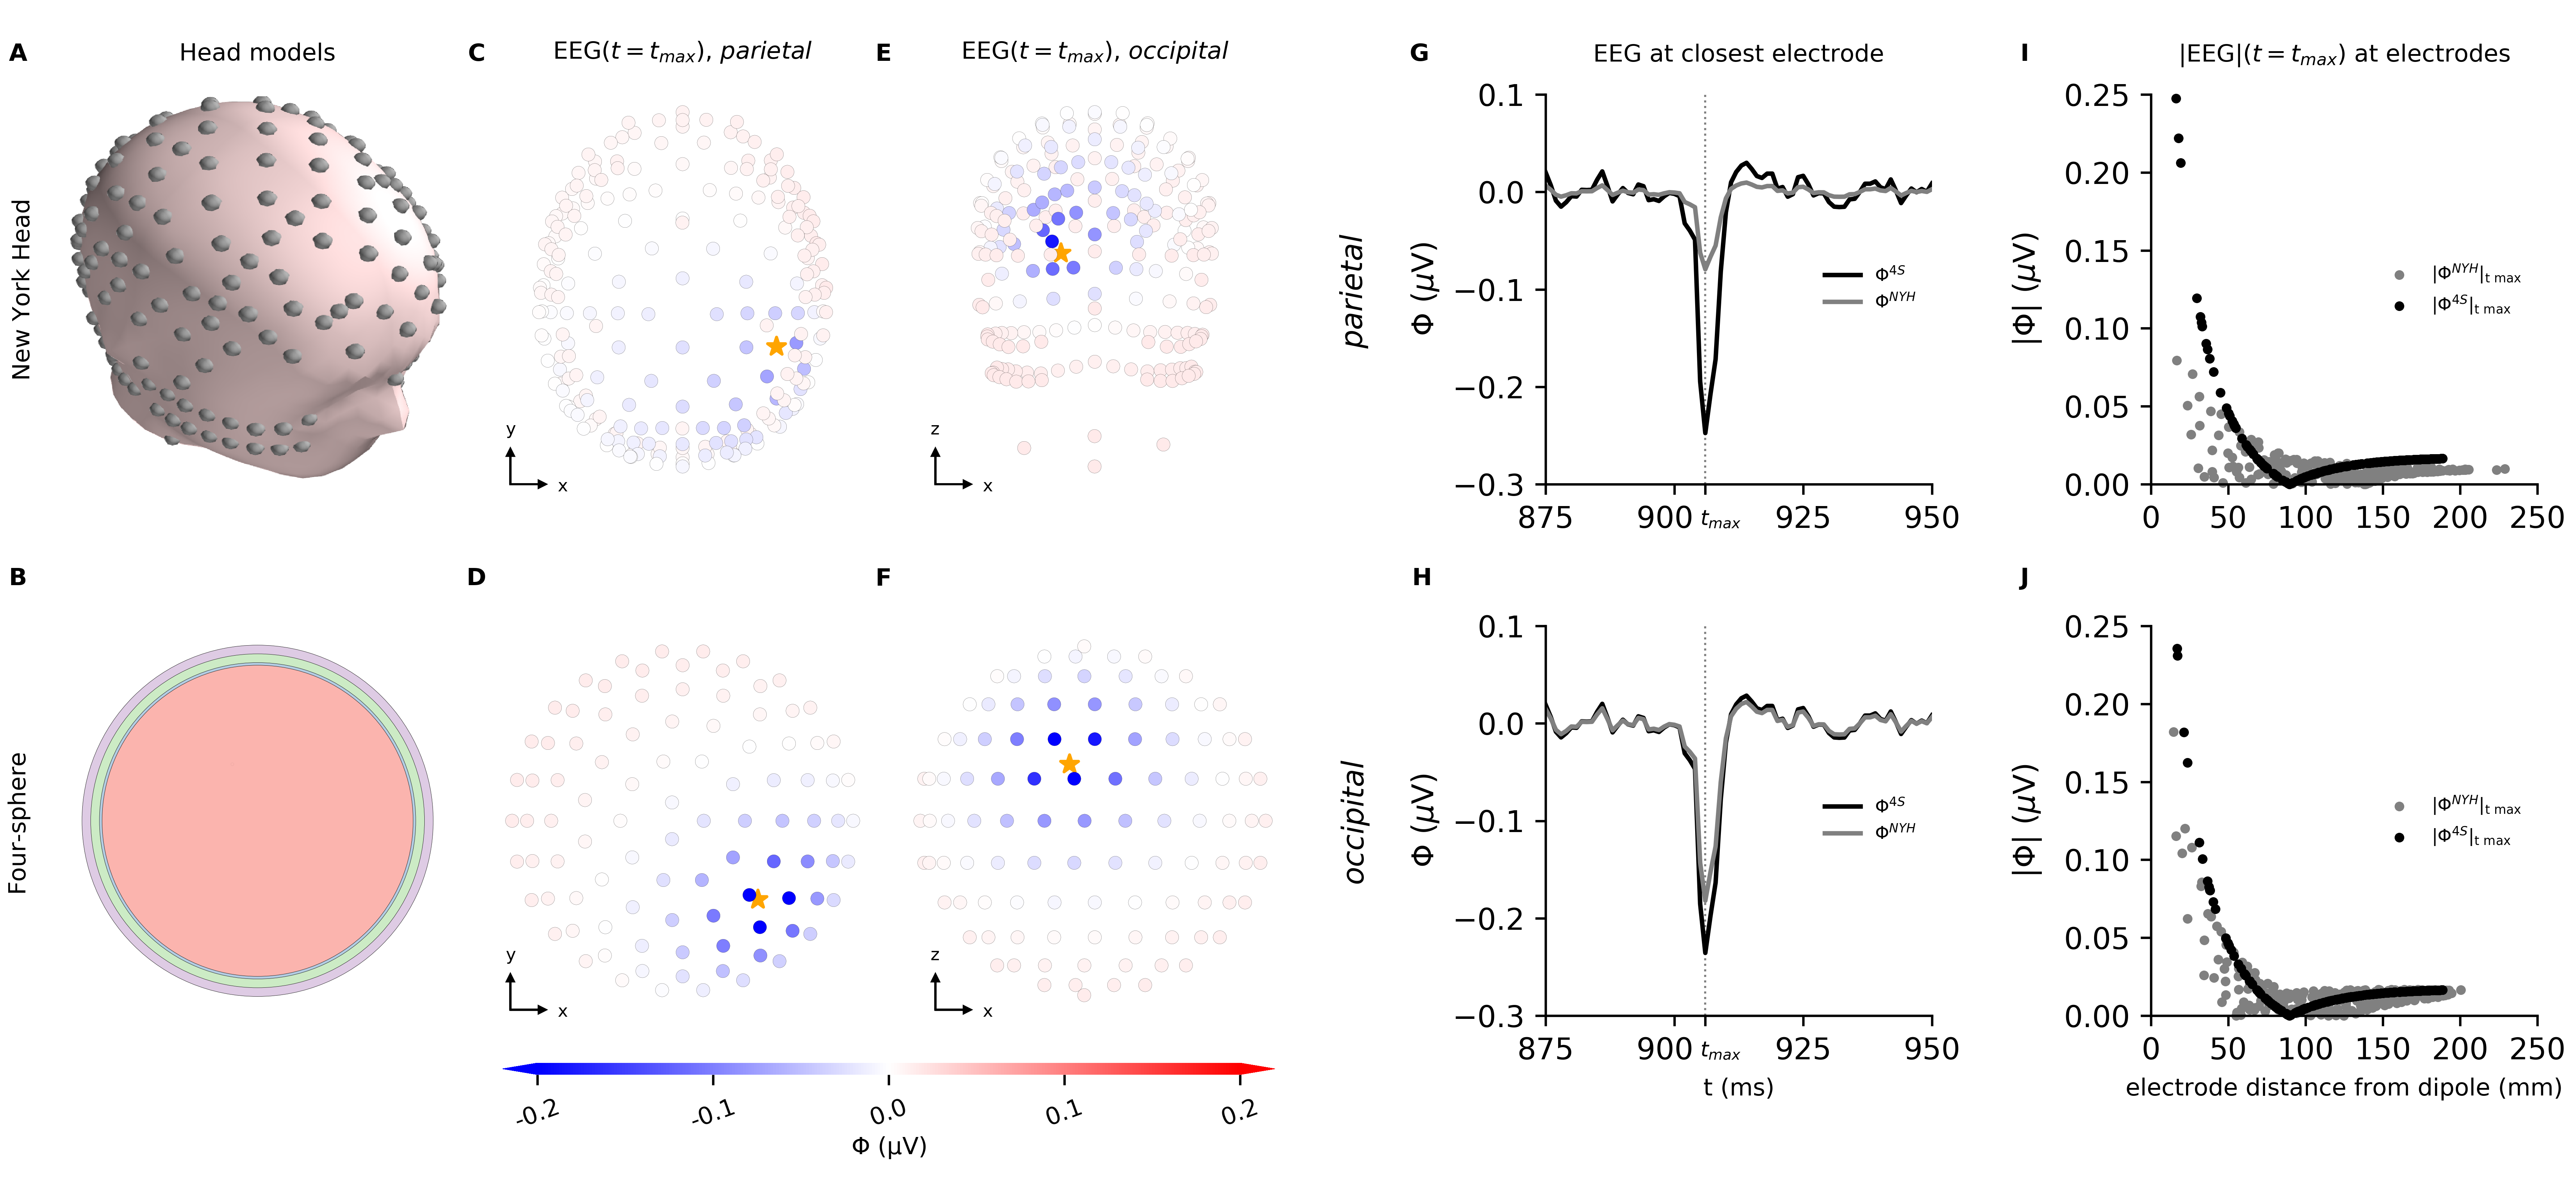
\includegraphics[width=1.0\textwidth]{figure6.png}
		\caption{\textbf{EEG signals from neuron population can be modeled with the four-sphere model and the New York Head}. EEG signals from population dipole resulting from waves of synaptic input to the cortical microcircuit model from \cite{POTJANS2014}. Population dipole was placed in two different locations: parietal lobe (C,D,G,I) and occipital lobe (E,F,H,J).
			{\bf A}: The New York Head model.
			{\bf B}: The four-sphere model consisting of four concentrical shells: brain tissue, CSF, skull and scalp. 
			{\bf C, D}: EEG signals ($\phi$) on scalp surface electrodes seen from above, showing timepoint of the strongest current dipole moment $|{\bf p}|$ of the population simulation. Dipole is placed in the parietal lobe and location is marked by orange star, having the following coordinates in the NYH model: (55, -49, 57)mm. EEG signals were computed with the New York Head model (C) and the four-sphere head model (D).
			{\bf E,F}: Equivalent to panel C,D however, dipole is placed in occipital lobe, and electrodes are seen from the back of the head. Dipole coordinates for NYH model: (-24.3, -105.4, -1.2)mm.
			{\bf G,H}: EEG trace computed with the four-sphere model and the New York Head model on closest scalp surface electrode: i.e. the electrode with the shortest distance to the current dipole moment location. G shows results for dipole placed in parietal lobe, while H shows results for dipole in occipital lobe.
			{\bf I}: Absolute value of EEG signals from panel C, D generated by dipole in parietal lobe, plotted as function of distance from dipole to measurement electrode.
			{\bf H}: Equivalent to panel I, however, EEG signals from panel E, F generated by dipole in occipital lobe.
			%	\snnote{The layout of this figure was meant to be pedagogical, as the rows, columns show the same model/ dipole location, but it's probably not compact enough..}
			%	\snnote{The same number of electrodes (224) in the four-sphere model for both dipole locations. Can try to optimize this, to get minimal distance between dipole and closest electrode.}
			%	\snnote{compute angle between EEG electrode and current dipole moment/ current dipole position vector. This should also affect the amplitude..}
		}
		%	\tvnnote{I see that tmax is marked, but I think it would be easier to see if we used ax.axvline(tmax, c='gray', ls=':') instead/in addition.}
		%	\tvnnote{Doesn't it make sense to show the time traces first before the max amplitude decay with distance?}
		\label{fig:compare_head_models}
	\end{figure}
	
	%\tvnnote{When we have a figure with a single current dipole of, say 1 nA/um, and corresponding EEG potentials, of say, 1 uV, we should send it to the New York Head model people (Stefan Haufe), and ask for a confirmation that the magnitude of the EEG in relation to the current dipole makes sense}
	%%%%%%%%%%%%%%%%%%%%%%%%%%%%%%%%%%%%%%%%%%%%%%%%%%%%%%%%%%%%%%%%%%%%%%%%
	%%%%%%%%%%%%%%%%%%%%%%%%%%%%%DISCUSSION%%%%%%%%%%%%%%%%%%%%%%%%%%%%%%%%%
	%%%%%%%%%%%%%%%%%%%%%%%%%%%%%%%%%%%%%%%%%%%%%%%%%%%%%%%%%%%%%%%%%%%%%%%%
	\section{Discussion}\label{sec:discussion}
	
	
	We have found that the single-cell current dipole moment is applicable for calculating a neuron's EEG-contribution, and that this approach can be helpful in estimating the relative EEG-contribution of different cell types and different modes of synaptic input, in addition to investigating 
	
	In this formalism it is easy to investigate the contribution to the EEG signal from, e.g., different cell types, from somatic spikes, or from dendritic spikes, by only comparing the z-component of the resulting current dipoles, without the need for the added complexity of head models etc.
	
	\begin{itemize}
		\item Good paper for discussion/intro:  \cite{COHEN2017} (``too little is done to understand the origin of the EEG'')
		\item Discuss value of results to ongoing large-scale simulation projects.
		\item ``EEG is hard to enterpret because of large number of neuron contributing''. True, but still basically (probably) just four main sources: apical excitation/inhibition and basal excitation/inhibition to pyramidal cells, and connectivity is to a large degree fixed, meaning that we could probalby map population firing rate to EEG.
		\item Discuss relevance to \cite{MAKI2019}?
		\item Discuss value of decoupling current dipole moments and head model
		\item Discuss kernel from population firing rates to current dipole moment?
		\item Discuss potential impact of I$_{\rm h}$ on human EEG \citep{NESS2016, NESS2018, KALMBACH2018}.
		\item Compare to other projects like HNN (Human Neocortical Neurosolver) (\url{https://hnn.brown.edu/}) and TVB \citep{TVB}
		\item Important work on the path towards a real understanding of the biophysical origin of EEGs \cite{BRUYNS2017}
	\end{itemize}
	On the other end of the scale are whole-brain simulations with  \citep{TVB}, to 
	\sntxt{
		\begin{itemize}
			\item Because of linearity, the EEG from a neural population is the sum of all the single-cell EEG contributions. However, if the spatial extent of the neural population (~ 1 mm) is small relative to the distance to the EEG electrodes (~ 1 cm), then individual current-dipoles can be summed, e.g., for each neural sub-population, or for the entire neural population, and the EEG signal can be computed based on the summed current dipoles. This could be a very promising approach for decomposing and understanding the EEG in large-scale neural  simulations like the cortical column simulations of the HBP, the Potians-Diesman  simulations of Hagen, or the Allen brain initiative.
			\item Which populations are important? We found that the EEG calculated as the sum of the single-cell EEG contributions from the current dipoles of all ~80,000 cells, spatially distributed within a cylinder (panel B and E) was indistinguishable from the EEG calculated as the sum of the EEG from 4 population current dipoles in the center of the population. Each of these 4 current dipoles was the sum of the z-components of the current dipoles of the pyramidal cells in the different layers (panel F, L23E, L4E, L5E, L6E). We found that all pyramidal cell populations had a substantial EEG contribution, however, the largest was the L2/3 population. It should however be noted that this is not a very realistic scenario, because of current-based synapses etc.
			
		\end{itemize}
		
	}
	
	% \appendix
	% \section{Point-Source vs. Line-Source Dipole Moment} \label{sec:point_line_cdm}
	% \tvnnote{I don't think we need to go into this.}
	% Considering the single-dipole neuron model, the line-source approximation gives a more accurate estimate than the point-source approximation. This section goes into the question of whether the choice of point-source or line-source approximation has an effect on the calculation of current dipole moments.
	% 
	% Transmembrane currents can be expressed as the spatial integral over the linear current density $i$. Following, the current dipole moment equation from transmembrane currents \eqref{eq:ptrans} is split into x-, y- and z- components, so that $\mathbf{p}(t) = p_x(t)\mathbf{\hat{x}} + p_y(t)\mathbf{\hat{y}} + p_z(t)\mathbf{\hat{z}}$, and each direction component is written as a function of $i$:
	% 
	% \begin{align}\label{eq:pxpypz}
	% p_x(t) &= \sum_{n=1}^N\int x_n i_n(x,t) dx, \nonumber\\
	% p_y(t) &= \sum_{n=1}^N\int y_n i_n(y,t) dy, \\
	% p_z(t) &= \sum_{n=1}^N\int z_n i_n(z,t) dz, \nonumber
	% \end{align}
	% where $N$ is the total number of compartments.
	% 
	% Next, an example for applying the point-source approximation to calculate the current dipole moment from a dendritic stick is outlined. We assume a straight multicompartmental dendrite model with $N$ compartments, each of length $\Delta L$, elongated in the z-direction only. Its linear current density for the point-source approximation can be expressed as follows
	% 
	% \begin{equation}
	% i_n(z,t) = I_n(t) \delta(z - z_n),
	% \end{equation}
	% where $I_n(t)$ is the space-independent current component and $z_n$ is the middle position of compartment $n$, i.e., where current can leave or enter. Plugging this into Equation \eqref{eq:pxpypz}, and integrating over the length of each compartment, $\Delta L$, the following expression for $p_z$ appears:
	% 
	% \begin{equation}
	% p_z = \sum_{n=1}^N \int_{z_n - \frac{\Delta{L}}{2}}^{z_n + \frac{\Delta L}{2}} z_n I_n(t) \delta(z - z_n)dz = \sum_{n=1}^N z_n I_n(t).
	% \end{equation}
	% 
	% When calculating the current dipole moment using the line-source approximation, the linear current density takes the following form:
	% \begin{equation}
	% i_n(z,t) = \frac{I_n(t)}{\Delta L}.
	% \end{equation}
	% Inserting this into Equation \eqref{eq:pxpypz} gives
	% 
	% \begin{align}
	% p_z
	% & = \sum_{n=1}^N \int_{z_n - \frac{\Delta L}{2}}^{z_n + \frac{\Delta L}{2}} z \frac{I_n(t)}{\Delta L}dz \nonumber \\
	% & = \sum_{n=1}^N \frac{I_n(t)}{\Delta L} \big[\frac{1}{2} z^2\big]_{z_n - \frac{\Delta L}{2}}^{z_n + \frac{\Delta L}{2}} \\
	% & = \sum_{n=1}^N z_n I_n(t). \nonumber
	% \end{align}
	% 
	% Hence, we have found that the point-source and the line-source approximations will give the exact same results when calculating current dipole moments. The simpler point-source approximation is therefore preferable.
	\section*{References}
	\footnotesize
	\bibliography{eeg_main}
\end{document}